\documentclass[12pt,a4paper]{report}
\usepackage[margin=1in]{geometry}
\usepackage{titlesec}
\usepackage{setspace}
\usepackage{hyperref}
\usepackage{graphicx}
\usepackage{xcolor}
\usepackage{float} % The [H] option used in figures comes from this package
\usepackage{sidecap} % Kept this package for now, but removed its specific environment use
\usepackage[font=footnotesize]{caption} % Options: scriptsize, footnotesize, small, normalsize
\captionsetup{position=top, font=small}
\usepackage{subcaption}
\usepackage{longtable}
\usepackage{array}

\setstretch{1.25}

% -------------------- Chapter and Section Formatting --------------------
\titleformat{\chapter}[hang]{\bfseries\LARGE}{\thechapter.}{1em}{} % Smaller than \huge
\titleformat{\section}[hang]{\bfseries\Large}{\thesection}{1em}{}
\titleformat{\subsection}[hang]{\bfseries\normalsize}{\thesubsection}{1em}{}

% -------------------- DOCUMENT --------------------
\begin{document}

% -------------------- TITLE PAGE --------------------
\begin{titlepage}
    \centering

    % --- Report Type ---
    \vspace*{1cm}
    {\Large \textbf{MTP STAGE-2 REPORT}}\\[1.5cm]

    % --- Main Title ---
    \begin{spacing}{0.75}
    {\fontsize{26}{38}\selectfont \textbf{Low-Cost Automated Tomato Sorting System}\par}
\end{spacing}

    \vspace{2cm}
    
\includegraphics[width=6cm]{iitb_logo.png}\\[3cm]

    \vfill % Pushes the author and guide info to bottom-left

    % --- Bottom Left: Author & Guide ---
    \begin{flushleft}
        {\large \textbf{Submitted by}}\\[0.3cm]
        {\Large \textbf{Jay Sonawane}}\\
        M.Tech, Computer Science and Engineering\\[1cm]

        {\large \textbf{Under the Guidance of}}\\[0.3cm]
        {\Large \textbf{Prof. Shivaram Kalyanakrishnan}}\\
    \end{flushleft}
\end{titlepage}

% -------------------- TABLE OF CONTENTS --------------------
\tableofcontents
\newpage


\chapter{Introduction}

MTP Stage-1 established a tomato ripeness classification pipeline using MobileNetV2. The work also investigated the effect of background standardization on classification accuracy and included a preliminary exploration of YOLO-based object detection using automatically generated annotations. The models were trained and evaluated on a curated dataset containing segmented images of individual tomatoes. Although this approach provided a useful starting point for the project, the images used during training and evaluation did not fully represent the conditions in which the system was eventually expected to operate.

In MTP Stage-2, the focus shifted towards deploying the system in the physical tomato sorting chamber and evaluating its performance under actual operating conditions. Unlike the curated dataset used in Stage-1, images captured inside the chamber contained the original background and the reflections produced by the mirror arrangement used in the setup. The camera therefore captured the actual scene rather than an isolated tomato against a standardized background. This introduced a difference between the images seen by the model during training and those encountered during deployment.

When the Stage-1 YOLO model was tested on images captured inside the actual chamber setup, its performance was significantly worse than its validation results had suggested. This indicated that good performance on the curated test dataset did not necessarily translate to reliable detection in the physical setup. The difference could not be addressed simply by training the same model for more epochs or increasing its size. A series of experiments was therefore conducted to identify the differences between the Stage-1 training images and the actual chamber images, and provided the basis for developing a more suitable dataset and detection pipeline.

Based on these observations, the data collection process was redesigned around the physical chamber. Images were captured using the chamber camera and its mirror arrangement, with the original background and lighting conditions retained. The dataset was extended to cover three ripeness categories: unripe, ripe, and overripe. Collecting data for the overripe category required additional effort because such tomatoes were relatively difficult to procure and maintain during the capture process. Multiple views of each tomato were collected so that the model could learn from the variations in appearance across the different camera views.

Preparing annotations for these full-frame images presented another challenge. Since each image could contain multiple visible instances of the tomato due to the camera and mirror arrangement, manually drawing bounding boxes for every image would have been time-consuming. To reduce this effort, an annotation pipeline based on the Segment Anything Model 2 (SAM2) was developed. It generated candidate masks for objects in the captured images, which were then filtered to retain the relevant tomato instances. The selected masks were converted into bounding-box annotations in the format required for YOLO training. The resulting annotations were also visually inspected, and images with unsuitable detections were excluded where necessary.

Using the newly collected and annotated dataset, a YOLO11n detection model was trained for the three ripeness classes. Since multiple images were captured for each tomato, randomly splitting individual frames could result in images of the same tomato appearing in both the training and validation sets. Such a split would not provide a reliable estimate of how the model performs on previously unseen tomatoes. The final dataset split was therefore performed at the tomato level. In addition to the held-out validation data, the model was evaluated on independently captured tomatoes to examine its ability to generalize beyond the original capture session.

The next part of the work focused on deploying the trained model on embedded hardware. A Raspberry Pi 4 Model B with 8 GB of RAM was used to evaluate whether the detection pipeline could operate outside the desktop GPU environment used during model development. The trained model was exported to a format suitable for deployment, and its predictions and inference time were compared across different execution environments. 

Apart from model deployment, the way inference was initiated was also considered. Running the detection model continuously would require unnecessary computation when the chamber was empty or when no new tomato was being processed. To address this, an event-triggered inference mechanism was developed. It monitors the chamber for the presence of a tomato and waits for the scene to become sufficiently stable before capturing the required views and running classification. This allows the model to perform inference in response to an actual event rather than processing every incoming camera frame continuously.

The work carried out in MTP Stage-2 therefore covers the transition from a model evaluated on curated images to a detection system tested under the conditions of the physical sorting chamber. It includes investigating the limitations of the earlier model, collecting and annotating a new dataset, training and evaluating a three-class detector, and deploying the model on embedded hardware. The event-triggered inference mechanism further explores how the detection pipeline can be operated as part of the setup.

\chapter{Summary of Stage-1}

This chapter provides a brief overview of the system developed during MTP Stage-1. It describes the initial hardware setup, the different modelling approaches that were explored, and the development of the detection pipeline. This background is useful for understanding the things carried out in Stage-2, which were motivated by limitations observed when the earlier model was tested in the physical sorting chamber.

\section{Problem and Hardware Setup}

The objective of the project is to automate the classification of tomatoes based on their ripeness, with the categories being unripe, ripe, and overripe. During Stage-1, a vertical cylindrical sorting chamber was developed in collaboration with the e-Yantra lab. The setup uses a camera along with a mirror arrangement that allows both a direct view and a mirrored view of the tomato to appear in a single captured frame. A roller mechanism is used to rotate the tomato, allowing images to be captured from different views. The setup also includes an Arduino-controlled feeder and sorting mechanism, which are intended to handle the movement and sorting of tomatoes.

\section{Model Iterations}

During Stage-1, three modelling approaches were explored, each addressing a different aspect of the classification and detection problem.

\textbf{Model A} used MobileNetV2 to classify raw tomato images without any preprocessing. It achieved approximately 89\% validation accuracy. However, further analysis indicated that the model was also learning features associated with the image background, rather than relying entirely on the appearance of the tomato. As a result, its predictions could be affected by changes in the background.

To address this issue, \textbf{Model B} introduced a background-standardization step before classification. A saturation threshold was used to identify the tomato region, and the remaining pixels were replaced with a solid black background. This reduced background variation across the training images and improved the validation accuracy to approximately 97\%. The approach provided better results on the curated dataset, although, as discussed in the diagnostic chapter of this report, it also introduced a dependence on the standardized background. This became an important consideration when the model was later tested on images captured inside the sorting chamber.

\textbf{Model C} explored a different approach based on object localization. It used segmentation to identify the tomato region and generate a bounding box around it. This approach was primarily used for visualization and exploration and was not carried forward for model training.

\section{Exploration of YOLO-Based Approach}

During Stage-1, a YOLO-based approach was also explored, given its widespread use in existing work. The objective was to investigate whether YOLO could be used for tomato localization and ripeness classification in the sorting system. Since the available dataset consisted of curated images of individual tomatoes, an automatic annotation pipeline was developed to prepare the dataset for training. The Segment Anything Model 2 (SAM2) was used in automatic mask-generation mode to obtain masks for the tomatoes in these images, avoiding the need for manual annotation. The generated masks were used to separate the tomatoes from their backgrounds and place them on a black canvas. Bounding boxes were then computed from the masks to generate annotations in the format required by YOLO.

The resulting dataset was used to train a YOLO11s model, which achieved a validation mAP50-95 of 0.995. While this indicated very high performance on the Stage-1 validation data, the model's performance on actual chamber footage was considerably different. The gap between the curated images used for training and the images captured inside the sorting chamber became an important issue during Stage-2.
\section{Mobile Deployment}

Alongside the detection experiments, the MobileNetV2 classifier developed in Model B was prepared for mobile deployment. The trained model was converted to TensorFlow Lite and integrated into a Flutter application, allowing predictions to be performed directly on the mobile device without requiring a continuous connection to a server. Since each captured frame contained both a direct and a mirrored view of the tomato, the application used a probability-fusion approach. The softmax probability outputs from the two views were averaged to obtain a single classification for the tomato. This allowed information from both views to contribute to the final prediction.

\chapter{Diagnosing the Stage-1 Model's Failure on Chamber Data}

This chapter presents the central diagnostic investigation of Stage-2: understanding why the Stage-1 YOLO model, despite reporting a validation mAP50-95 of 0.995, failed when evaluated on images captured from the physical sorting chamber.

\section{Initial Observation: Live Chamber Failure}

The Stage-1 YOLO11s model was first evaluated by running it live against the chamber's camera feed. Two failures were observed immediately. First, pointing the camera at a completely empty chamber produced a confident detection (class ``unripe'', confidence 0.97) where no tomato was present at all. Second, when a genuinely ripe tomato was placed in the chamber, the model frequently misclassified it as unripe or overripe rather than ripe. This contradicted the model's reported validation performance and indicated that the 0.995 mAP50-95 figure did not reflect how the model would behave in actual deployment.
\begin{figure}[H]
\centering
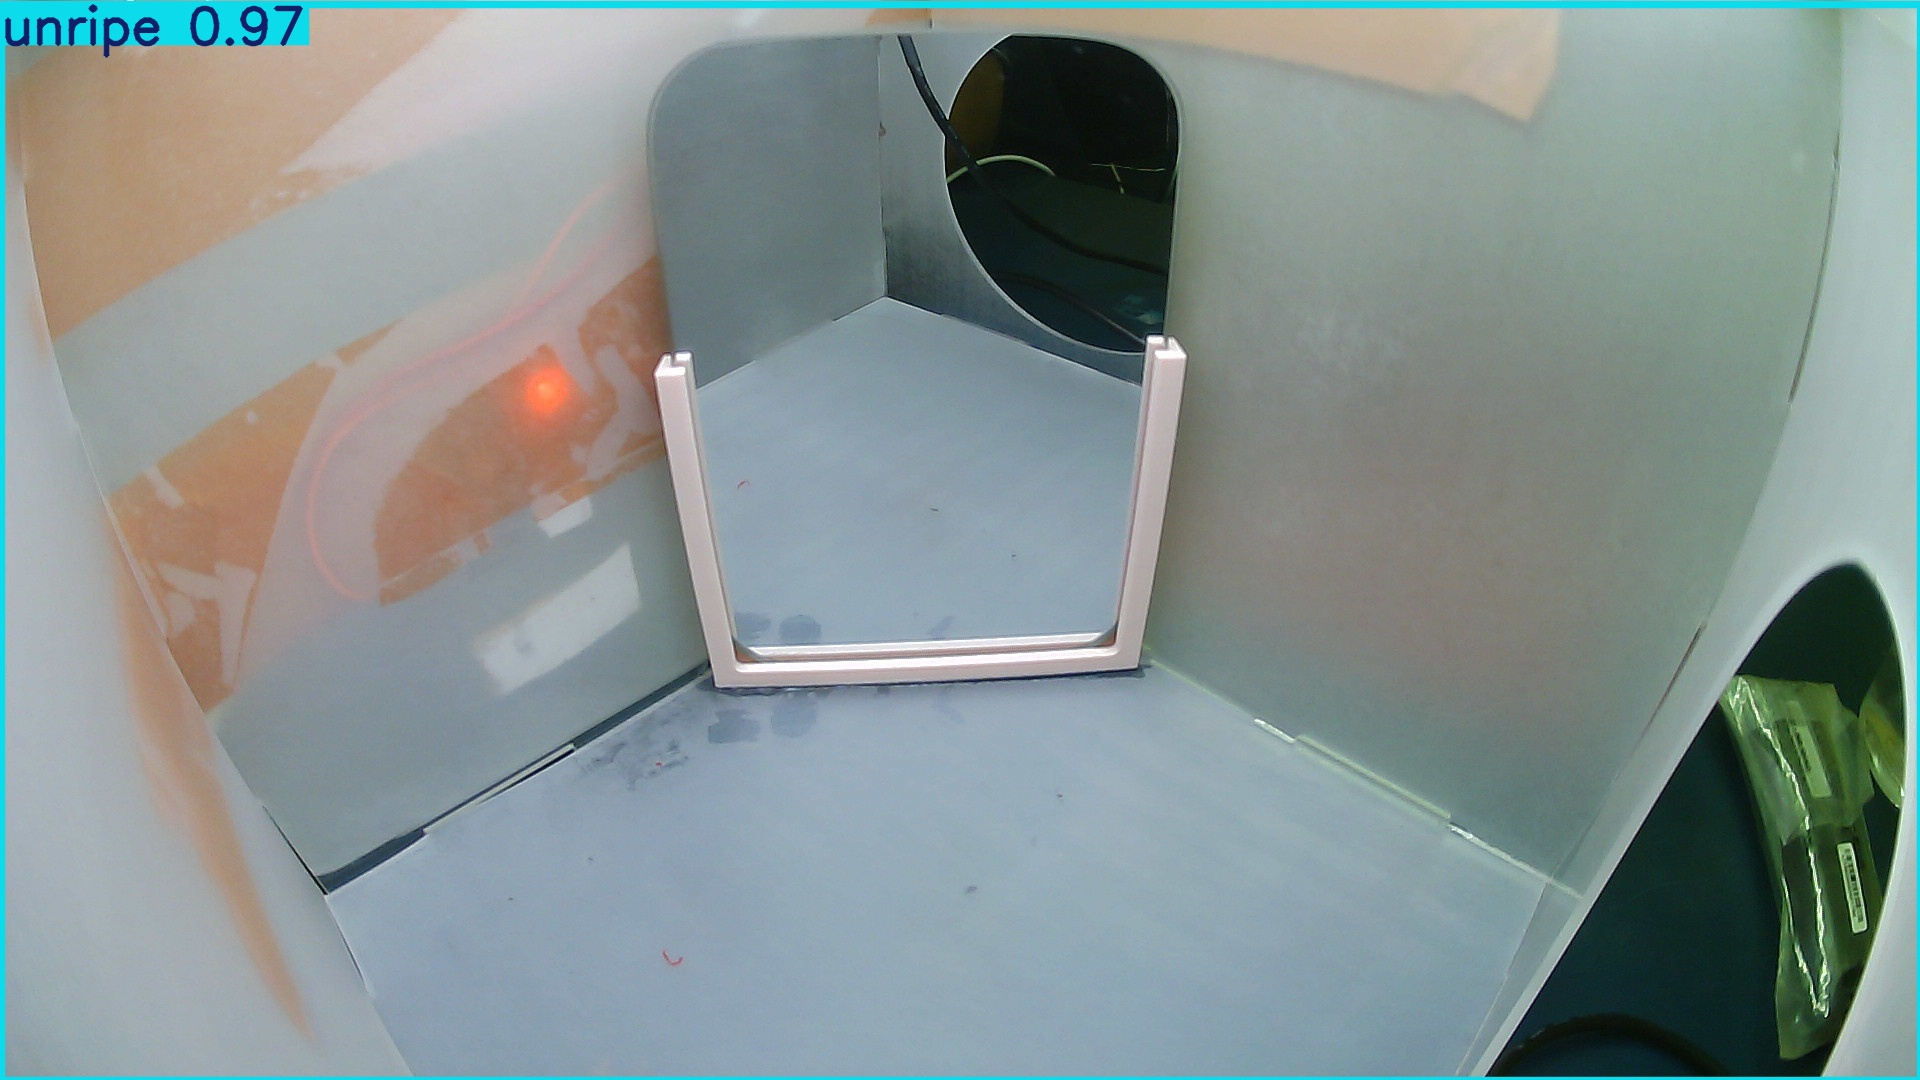
\includegraphics[width=0.8\linewidth]{images/diagnosis_empty_chamber.jpg}
\caption{Empty chamber}
\end{figure}

\begin{figure}[H]
\centering
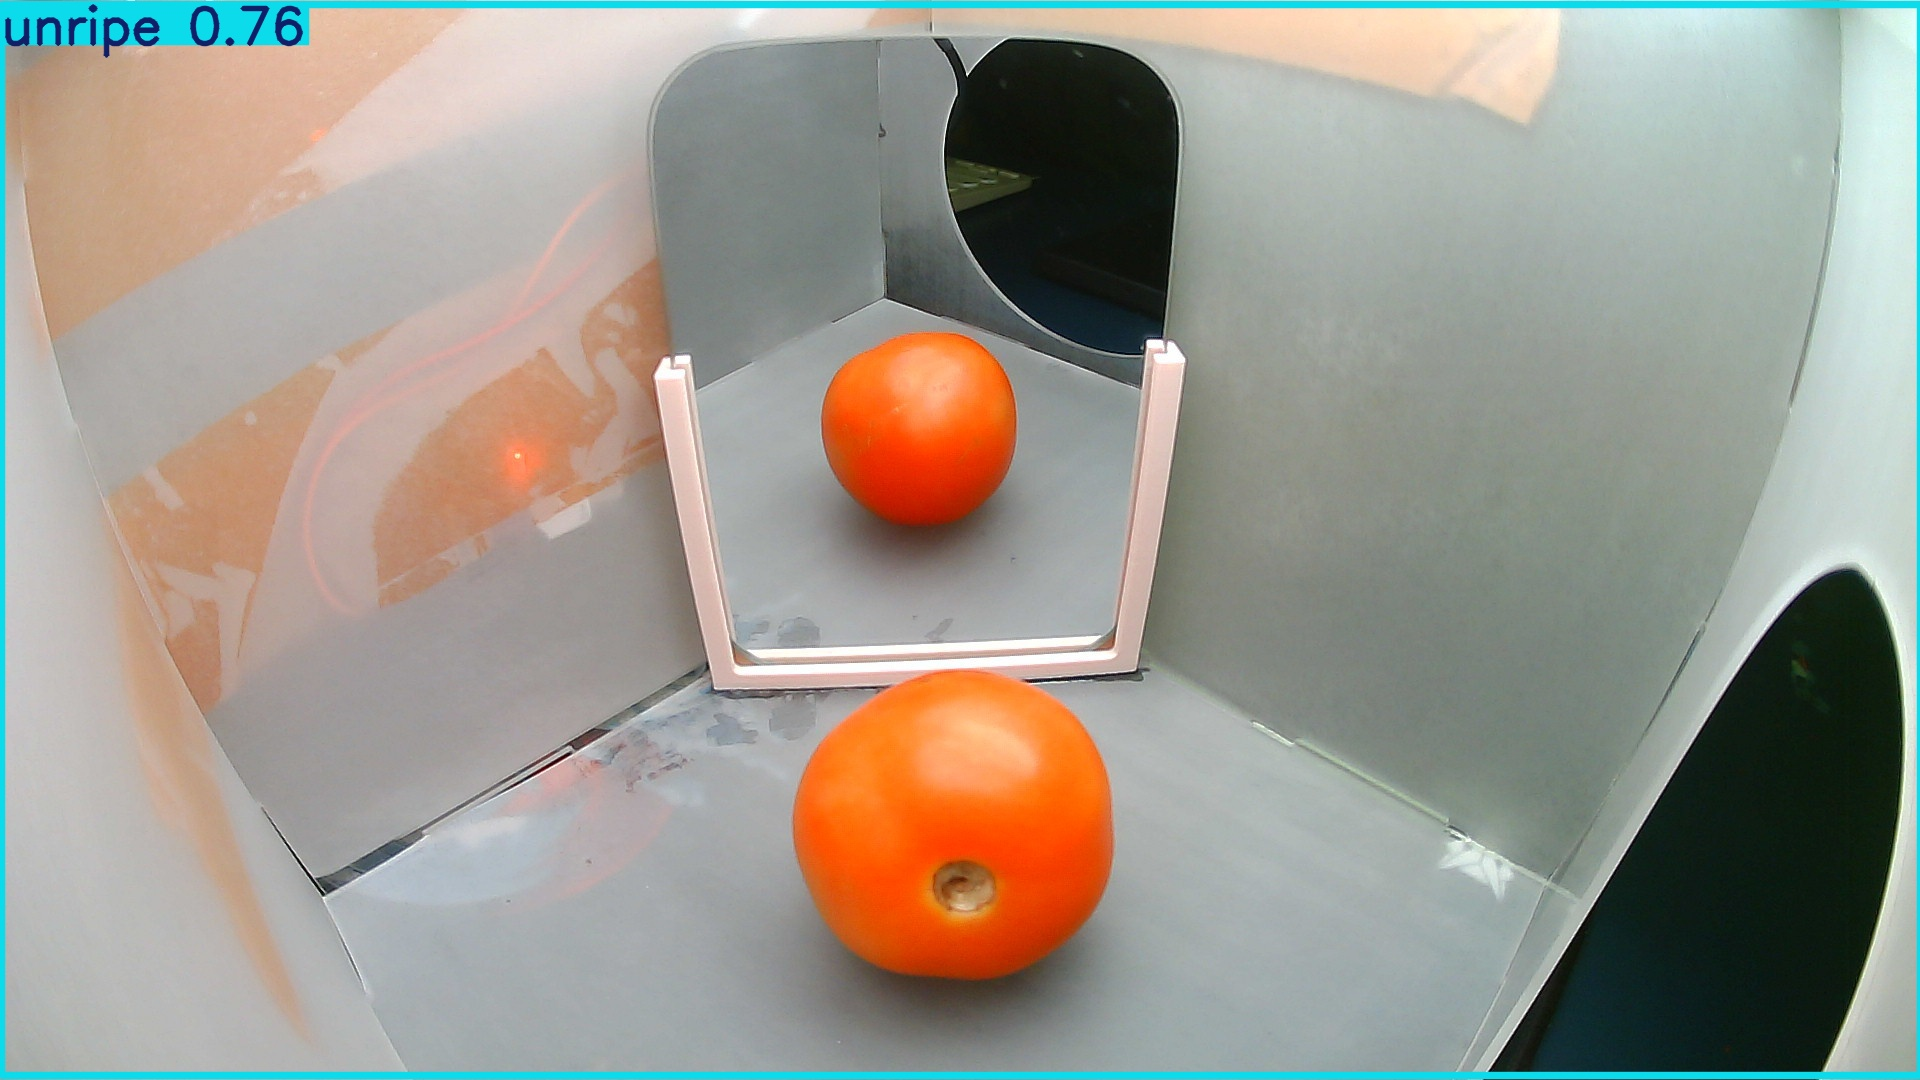
\includegraphics[width=0.8\linewidth]{images/diagnosis_ripe_misclassified.jpg}
\caption{Ripe tomato, misclassified}
\end{figure}
\section{Ruling Out Background Alone}

Another possible explanation was that the model was failing because of the difference in backgrounds. During Stage-1, the tomatoes were presented against a solid black background, whereas the chamber images contained grey walls, the mirror, and other elements of the physical setup. To investigate whether this background difference was responsible for the poor performance, the same chamber images were re-segmented using SAM2, and the resulting tomato regions were composited onto a black background. The original image resolution and tomato size were retained, without cropping or resizing the images. This allowed us to examine the effect of changing the background while keeping the original chamber framing unchanged.

If the background difference were the only reason for the failure, restoring the black background should have improved the model's performance. However, the opposite was observed. The ripe-class accuracy dropped to 0\%, with every ripe tomato being classified as ``overripe'' at confidence scores between 96\% and 98\%.

This result showed that the background difference alone could not explain the model's failure. In fact, removing the original chamber background made the classification of ripe tomatoes even worse. This suggested that other differences between the training images and chamber footage, particularly the appearance of the tomatoes, were also affecting the model's predictions.
\begin{table}[H]
\centering
\caption{Ripe-class accuracy on real chamber images, by model size}
\begin{tabular}{|l|c|c|}
\hline
\textbf{Model} & \textbf{Parameters} & \textbf{Ripe accuracy (chamber images)} \\
\hline
YOLO11n & $\approx$2.6M & 20.8\% \\
YOLO11s & $\approx$9.4M & 18.8\% \\
\hline
\end{tabular}
\end{table}

Both models failed on the ripe class to a similar degree, with the larger model performing marginally worse, not better. This rules out model capacity as the cause of the failure: a model-size explanation would predict the larger model should perform noticeably better, which was not observed.

\section{Identifying the Dataset Mismatch}

The consistent and highly confident misclassifications observed in the previous experiment suggested that the model was relying on visual features learned from the Stage-1 training dataset. A closer look at how the two datasets were collected provided an important clue. The Stage-1 dataset had been assembled from multiple sources, including images obtained from GitHub repositories and other publicly available sources. As a result, the tomatoes in the dataset could vary in their appearance, and the conditions under which the images were captured were not consistent.

For Stage-2, a new set of tomatoes was procured from market, and their images were captured using the physical classification chamber. This provided greater control over the data collection process and ensured that the images represented the conditions in which the system was intended to operate. However, it also revealed a noticeable difference between the appearance of tomatoes in the earlier dataset and those captured now.

\begin{figure}[H]
\centering

\begin{subfigure}[t]{0.3\linewidth}
    \centering
    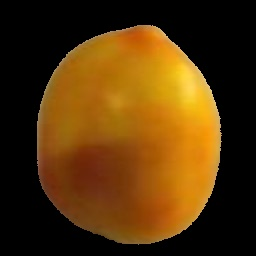
\includegraphics[height=4cm,keepaspectratio]{images/stage1_ripe_example.jpg}
    \caption{Stage-1 training,\\ ``ripe''}
\end{subfigure}
\hfill
\begin{subfigure}[t]{0.3\linewidth}
    \centering
    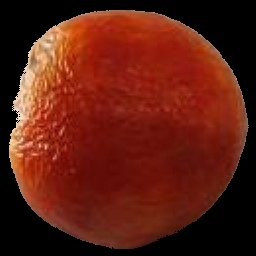
\includegraphics[height=4cm,keepaspectratio]{images/stage1_overripe_example.jpg}
    \caption{Stage-1 training,\\ ``overripe''}
\end{subfigure}
\hfill
\begin{subfigure}[t]{0.3\linewidth}
    \centering
    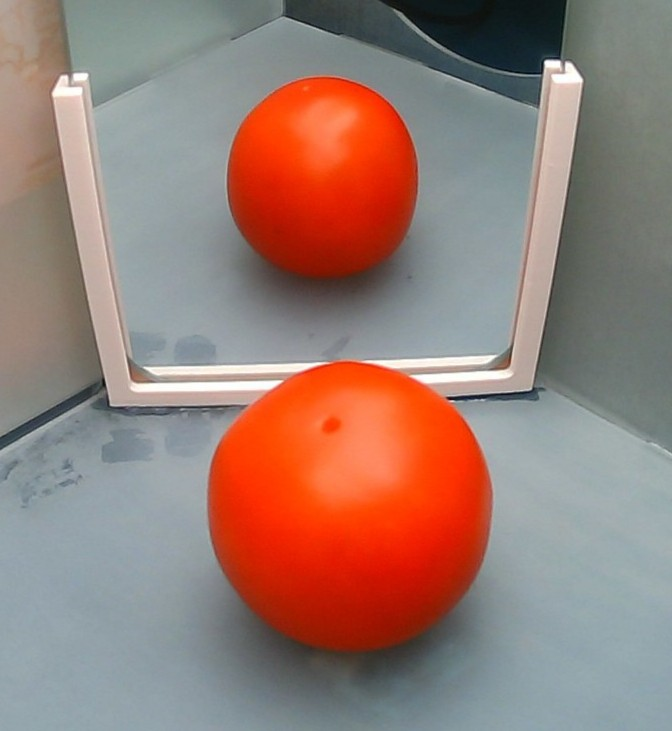
\includegraphics[height=4cm,keepaspectratio]{images/chamber_ripe_fullframe.jpg}
    \caption{Stage-2 chamber-captured\\ ripe tomato}
\end{subfigure}

\caption{Comparison of tomato appearance in the Stage-1 dataset and the Stage-2 chamber-captured data.}
\label{fig:domain-gap}
\end{figure}

As seen in Figure~\ref{fig:domain-gap}, the ripe tomatoes in the Stage-1 dataset predominantly have a dull orange or amber appearance. In contrast, the ripe tomatoes procured for Stage-2 and captured inside the classification chamber have a more vivid and saturated red appearance. Interestingly, this appearance is closer to that of the tomatoes labelled as ``overripe'' in the Stage-1 dataset. This difference in appearance could explain why the model frequently classified genuinely ripe tomatoes from the chamber as overripe. The model had learned the relationship between tomato appearance and ripeness labels from a dataset whose visual characteristics did not adequately represent the tomatoes encountered during actual deployment.

This also helps explain why the unripe class remained relatively robust in both the live-chamber test and the black-background re-test. Unripe tomatoes are predominantly green, whereas ripe and overripe tomatoes have shades of red and orange. The visual difference between unripe and ripe tomatoes is relatively large, while distinguishing ripe from overripe tomatoes depends on finer variations in colour. The differences between the two datasets therefore had a greater impact on the distinction between ripe and overripe tomatoes, which is consistent with the observed misclassifications.

\section{Localization as a Compounding Factor}

Apart from the differences in tomato appearance, there was also a significant difference in how tomatoes were represented in the Stage-1 training images and the actual chamber footage. During Stage-1, the YOLO model was trained on images containing a single tomato, which occupied almost the entire frame. The bounding boxes consequently covered roughly 70--80\% of the image. Figure~\ref{fig:stage1-localization} shows examples of the training images and their corresponding bounding boxes.

\begin{figure}[H]
\centering

\begin{subfigure}[t]{0.3\linewidth}
    \centering
    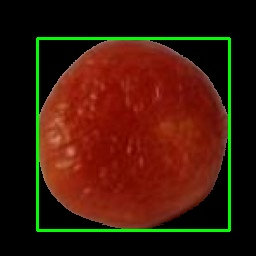
\includegraphics[height=4cm,keepaspectratio]{images/o (1958).jpg}
    \caption{Overripe}
\end{subfigure}
\hfill
\begin{subfigure}[t]{0.3\linewidth}
    \centering
    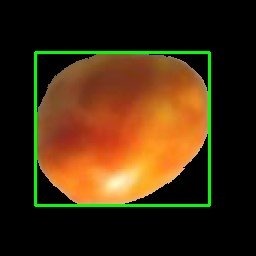
\includegraphics[height=4cm,keepaspectratio]{images/r (1599).jpg}
    \caption{Ripe}
\end{subfigure}
\hfill
\begin{subfigure}[t]{0.3\linewidth}
    \centering
    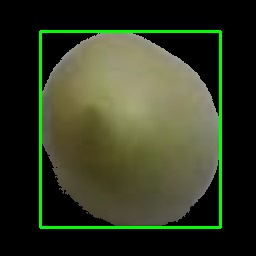
\includegraphics[height=4cm,keepaspectratio]{images/u (951).jpg}
    \caption{Unripe}
\end{subfigure}

\caption{Examples of Stage-1 training images showing individual tomatoes and their YOLO bounding-box annotations.}
\label{fig:stage1-localization}
\end{figure}

In contrast, the chamber camera captures a much wider scene containing both the direct view of the tomato and its reflection in the mirror. Each of these instances occupies a considerably smaller portion of the frame. The model therefore encountered a different localization problem during deployment: instead of detecting a large, isolated tomato, it had to locate smaller tomato instances within a wider scene containing the chamber background and hardware. This difference in object scale and framing made localization more challenging and further contributed to the poor performance of the Stage-1 model on real chamber footage.
\section{Summary of the Diagnosis}

The experiments and visual comparisons helped identify two major differences between the Stage-1 training data and the actual chamber footage. The first was the difference in tomato appearance. The Stage-1 dataset had been collected from multiple sources, and the appearance of tomatoes, particularly those belonging to the ripe class, differed from the tomatoes procured and captured during Stage-2. This affected the model's ability to distinguish between ripe and overripe tomatoes. The second difference was in object scale and framing. The Stage-1 YOLO model was trained on images containing a single tomato that occupied most of the frame, whereas the chamber camera captured a wider scene containing both the direct view and the mirror reflection of the tomato.

The model-size comparison showed that increasing the model size did not improve its performance on chamber images. Similarly, the black-background re-test showed that the background difference alone could not explain the failure. Together, these observations indicated that the Stage-1 model had learned from a dataset that did not adequately represent the appearance and spatial arrangement of tomatoes in the actual sorting chamber.

These findings motivated the data collection and annotation approach adopted in Stage-2. Instead of relying on images collected from different sources and training on isolated, background-removed tomato images, a new dataset was collected using tomatoes procured specifically for the project and captured inside the physical sorting chamber. The full chamber images were retained for annotation and model training so that the resulting model could be trained on data that more closely represented its intended deployment environment.

\chapter{Chamber Dataset Collection and Annotation}

This chapter describes the data collection protocol used to capture real chamber images for all three ripeness classes, and the automated annotation pipeline built to label them without requiring manual bounding-box annotation.

\section{Capture Protocol}

Images were captured using the existing camera and mirror arrangement in the sorting chamber. The white LED lighting was kept at a fixed preset throughout the capture process to maintain consistent lighting conditions. For each tomato, six frames were captured at different rotation positions, providing multiple views of the same tomato rather than relying on a single image. Each captured frame contained two visible instances of the tomato: the direct view and its reflection in the mirror, as in the original chamber setup developed during Stage-1.

\begin{table}[H]
\setlength{\intextsep}{8pt}
\centering
\begin{tabular}{|l|c|c|c|}
\hline
\textbf{Class} & \textbf{Tomatoes captured} & \textbf{Positions per tomato} & \textbf{Total frames} \\
\hline
Ripe & 11 & 6 & 66 \\
Unripe & 7 & 6 & 42 \\
Overripe & 8 & 6 & 48 \\
\hline
\end{tabular}
\caption{Summary of images captured for each ripeness class}
\label{tab:capture-summary}
\end{table}
\vspace{-1em}

Collecting overripe tomatoes was particularly challenging, as they were difficult to procure. To address this, some of the tomatoes initially used for collecting the ripe-class images were kept until they ripened further and were then used for capturing the overripe-class images.
\section{Automated Full-Frame Annotation using SAM2}

Unlike the Stage-1 pipeline, which worked with a single pre-cropped tomato in each image, Stage-2 required annotations for two tomato instances within each full chamber image: the direct view and its reflection in the mirror. To automate this process, the Segment Anything Model 2 (SAM2) was used in automatic mask-generation mode. This allowed candidate object masks to be generated across the entire image without requiring manual clicks or bounding-box prompts for individual images.

However, SAM2 does not specifically recognize tomatoes. It generates masks based on visual features such as object boundaries, shape, and texture. As a result, the initial outputs sometimes included parts of the chamber hardware, such as the mirror frame and its mounting structure, along with the actual tomatoes. Some filtering was therefore required to identify the two relevant instances reliably.

A colour-based filtering step was introduced to eliminate these unwanted candidates. The pixels within each candidate mask were examined to determine whether their colours fell within a suitable hue range for tomatoes. Red and orange shades were considered for ripe and overripe tomatoes, while green and yellow shades were considered for unripe tomatoes. A minimum saturation threshold was also applied to reject candidates corresponding to grey surfaces, such as the mirror frame and chamber walls. Their bounding boxes were then extracted and converted into normalized YOLO-format annotations.

\begin{figure}[!htbp]
    \centering

    \begin{subfigure}[t]{0.46\linewidth}
        \centering
        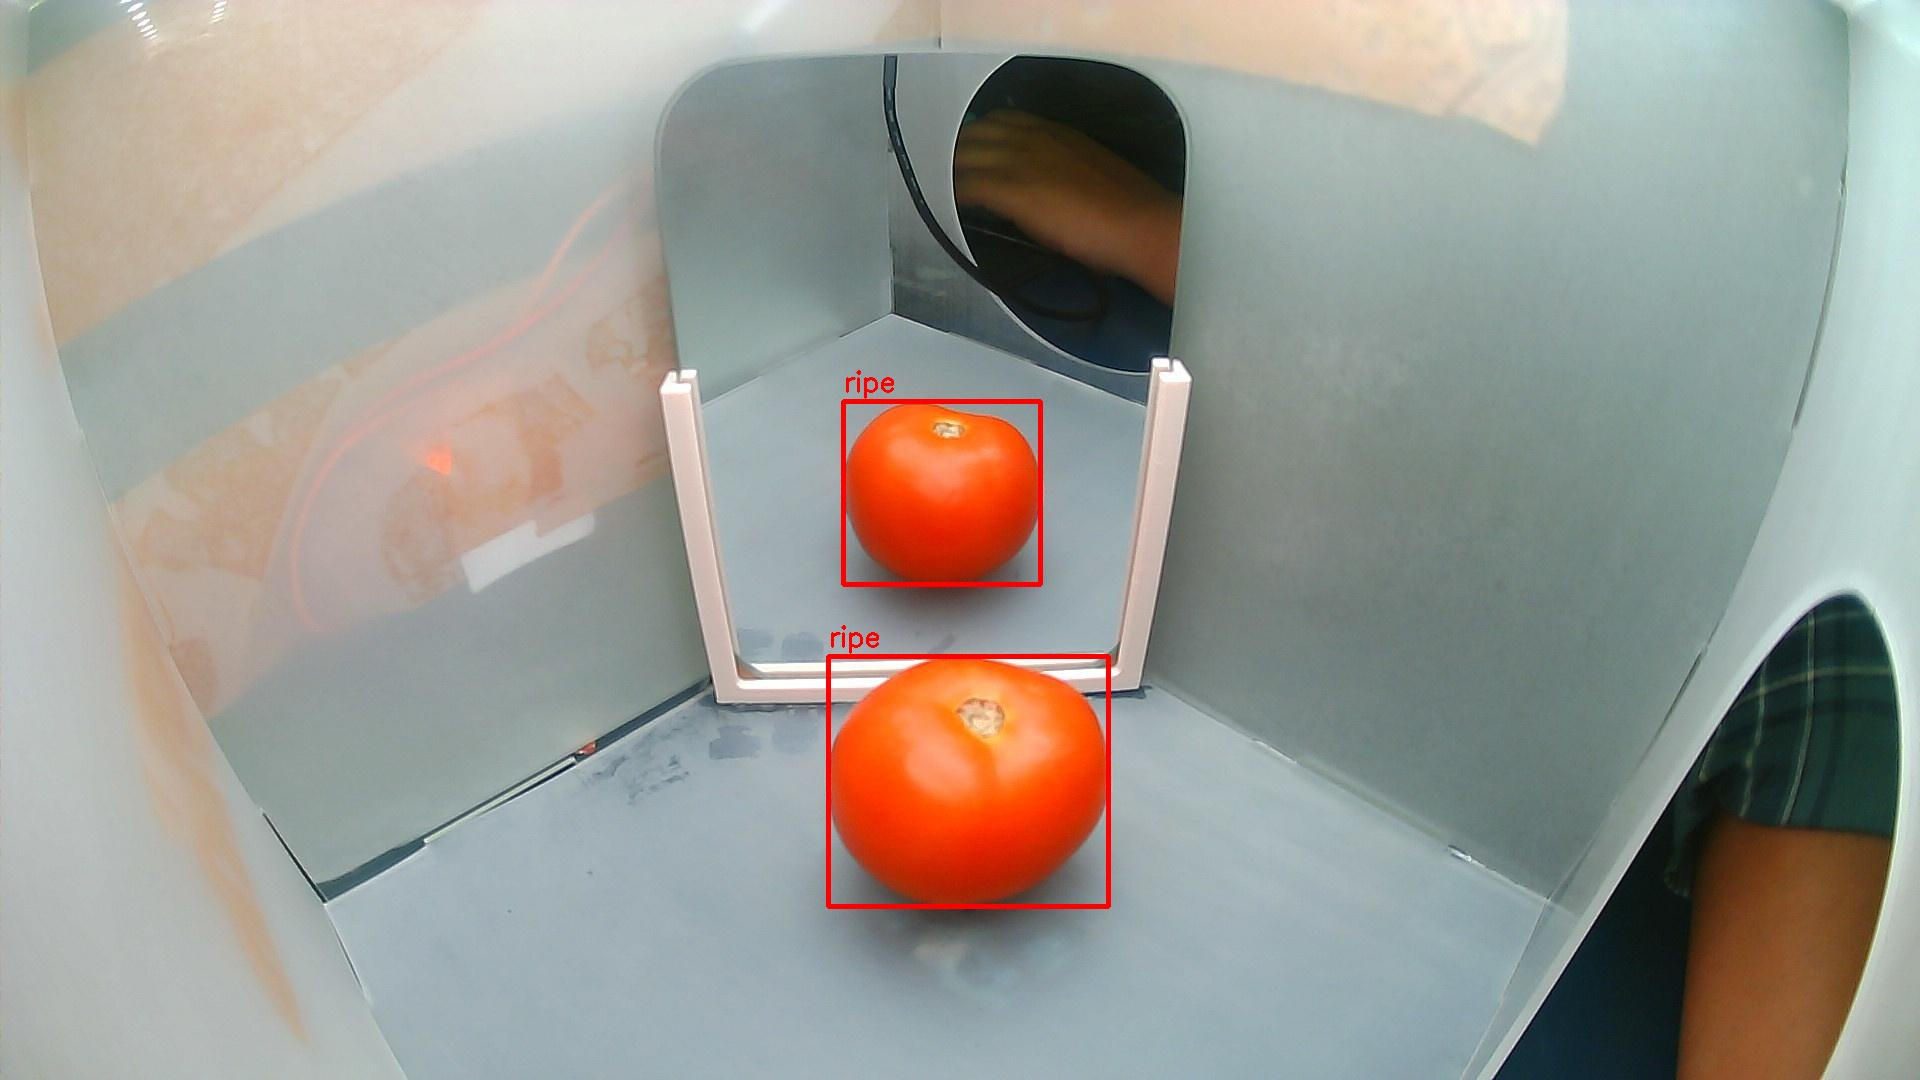
\includegraphics[width=\linewidth,height=4.2cm,keepaspectratio]{images/sam_ripe.jpg}
        \caption{Ripe}
    \end{subfigure}
    \hfill
    \begin{subfigure}[t]{0.46\linewidth}
        \centering
        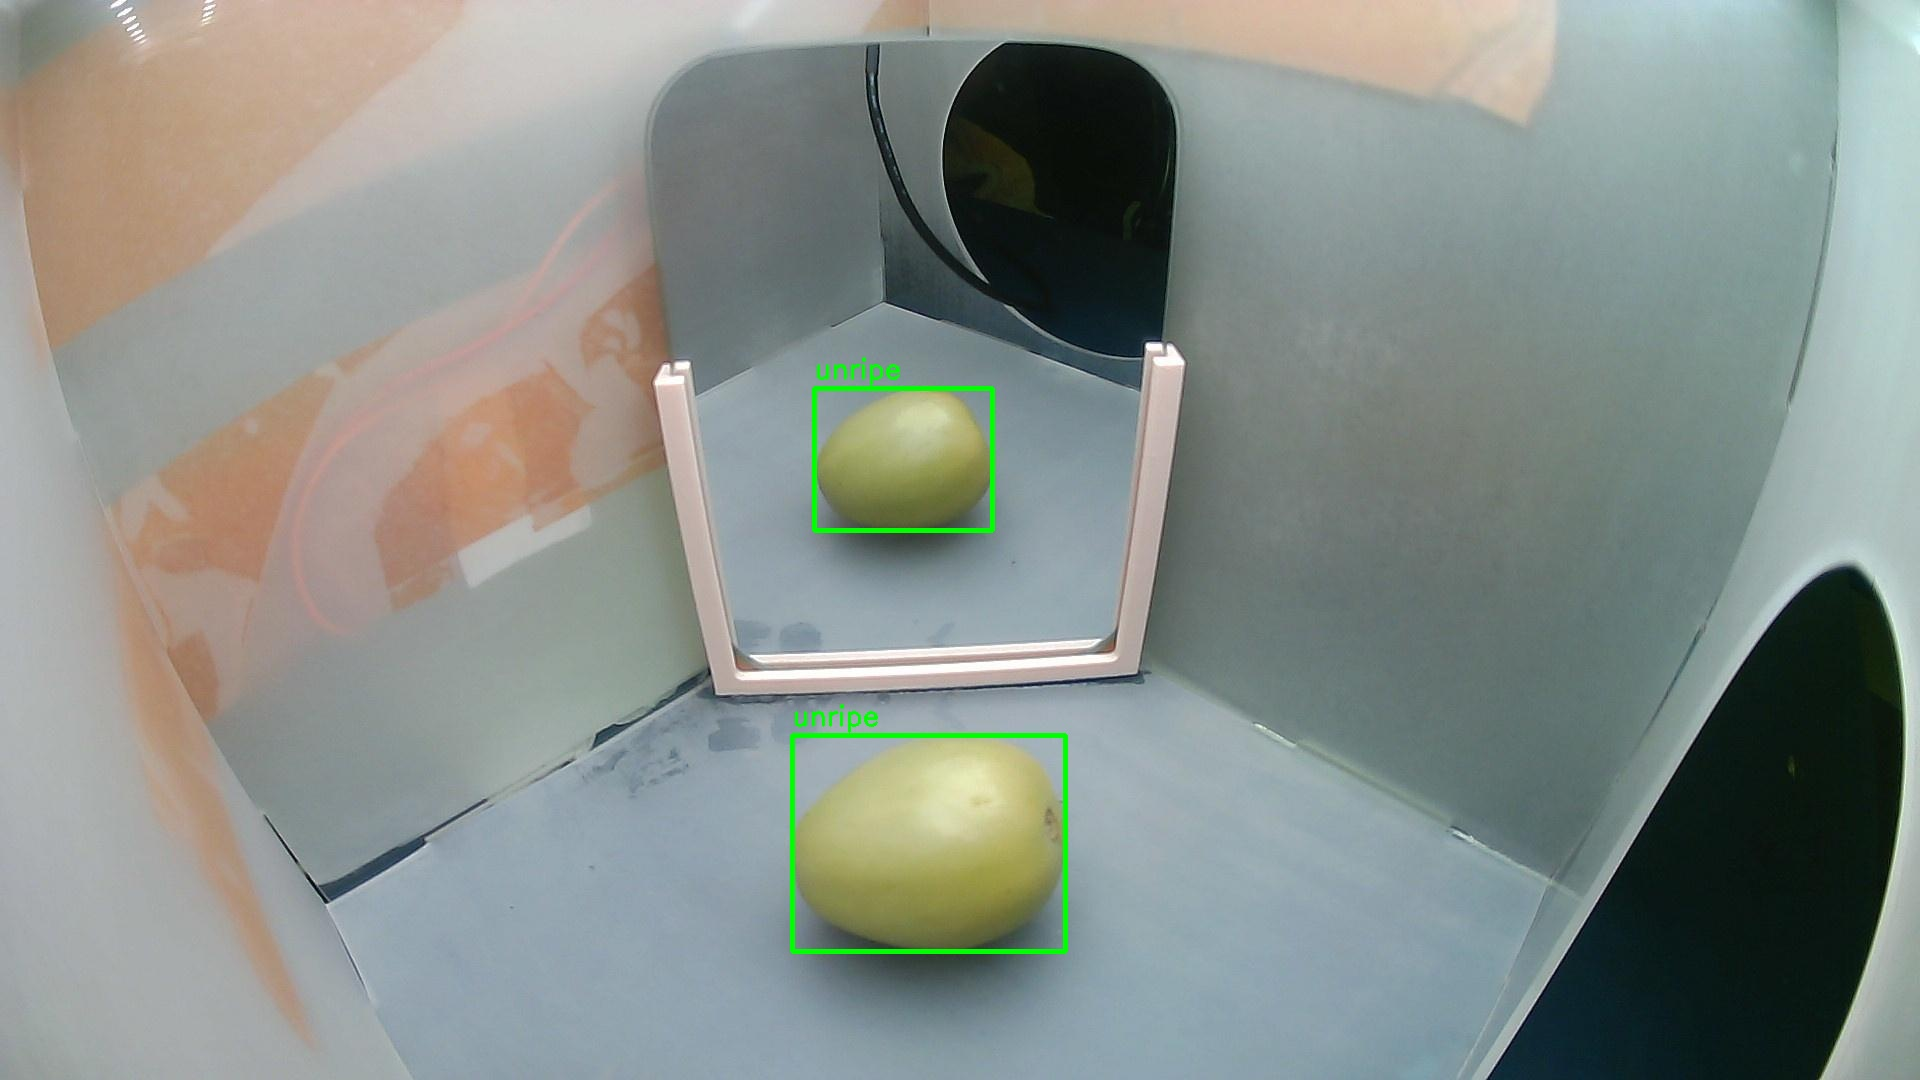
\includegraphics[width=\linewidth,height=4.2cm,keepaspectratio]{images/sam_unripe.jpg}
        \caption{Unripe}
    \end{subfigure}

    \vspace{0.2cm}

    \begin{subfigure}[t]{0.46\linewidth}
        \centering
        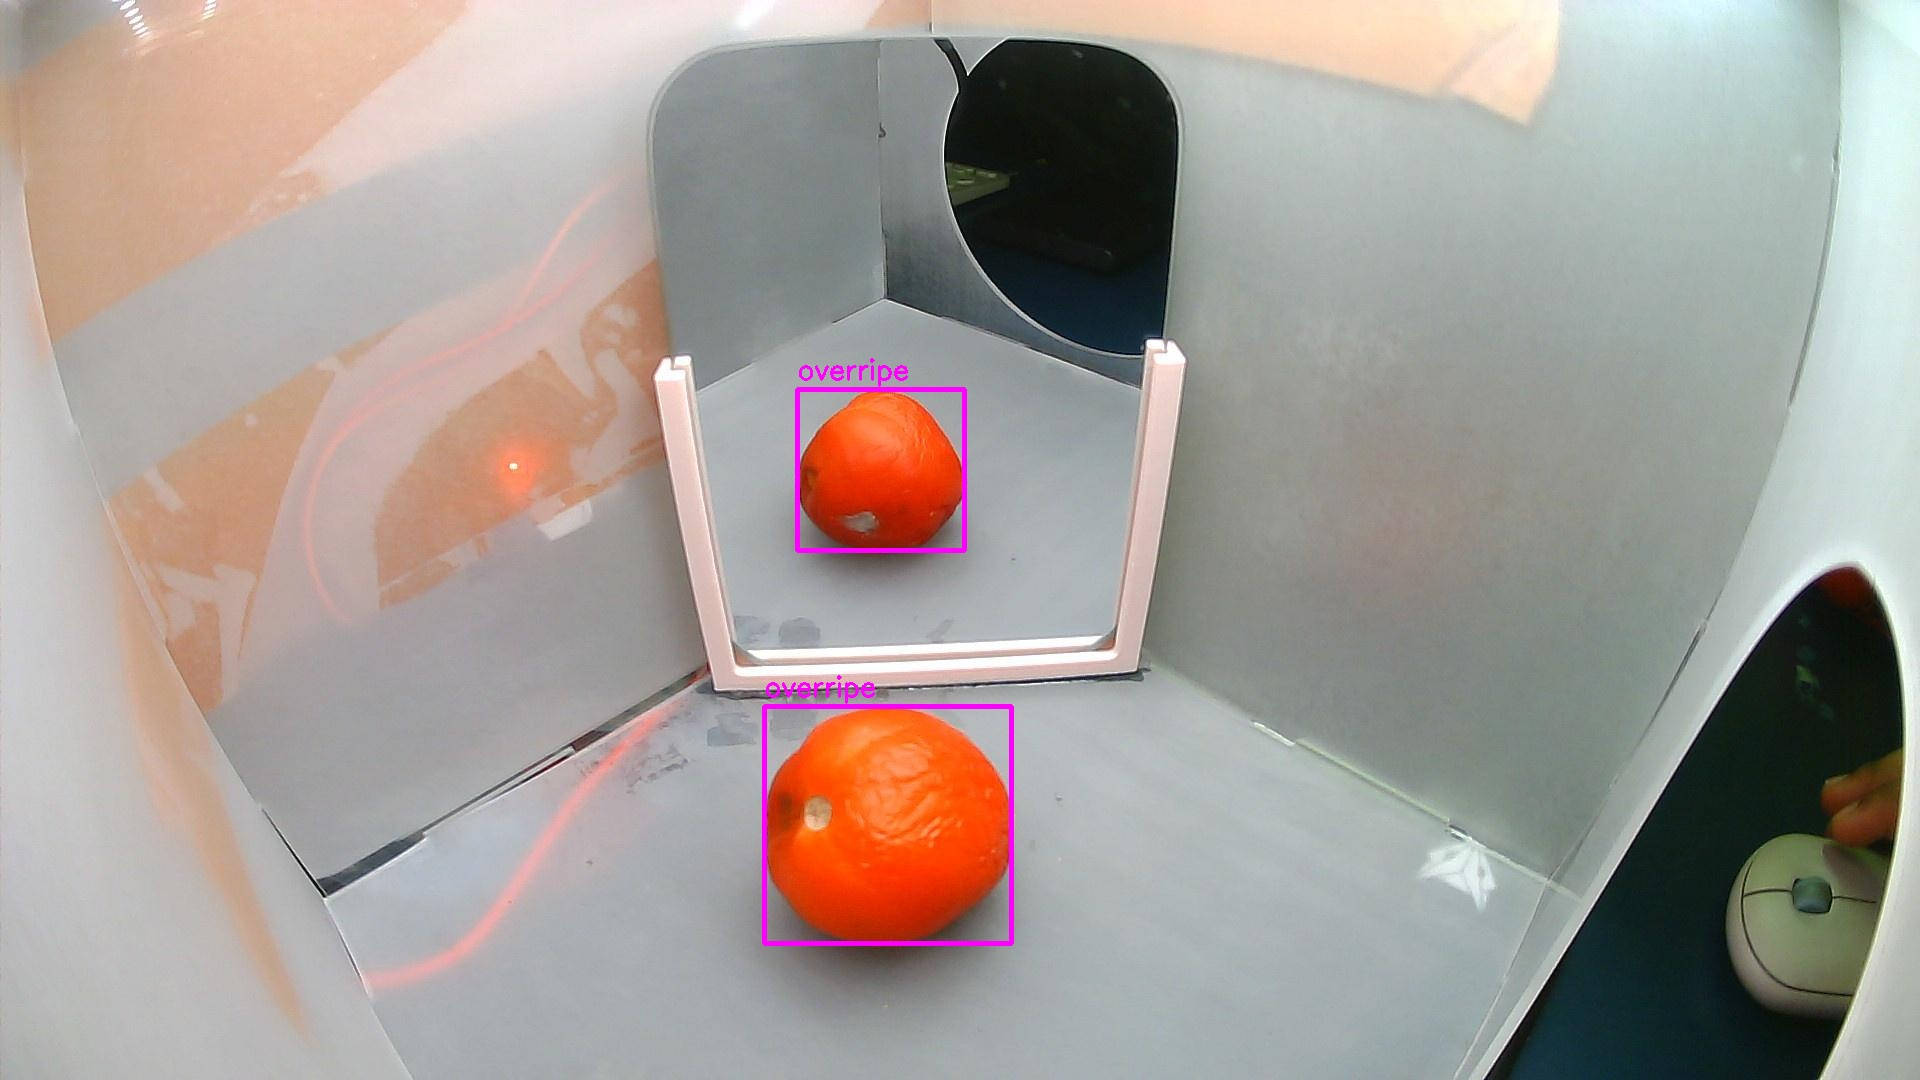
\includegraphics[width=\linewidth,height=4.2cm,keepaspectratio]{images/sam_overripe.jpg}
        \caption{Overripe}
    \end{subfigure}

    \caption{Examples of SAM2-generated bounding-box annotations on full chamber images.}
    \label{fig:sam-annotations}
\end{figure}
Figure~\ref{fig:sam-annotations} shows examples of the generated annotations for all three ripeness classes. Both the direct and mirror-view instances are localized within the same image, while the original chamber background is retained. This differs from the Stage-1 annotation pipeline, where the tomato was separated from its background and placed on a black canvas.

The annotation pipeline was not successful for every frame. In a small number of cases, the colour filter rejected one of the tomato instances because its colour distribution did not sufficiently match the selected range. Such frames were identified through visual inspection and discarded rather than corrected manually. Since only a small fraction of the collected frames was affected, this approach was used to maintain consistency in the automatically generated annotations.
\section{Chamber Lighting as a Dataset Variable}

The diagnosis highlighted the importance of maintaining consistent visual conditions when collecting the chamber dataset. In particular, since the model's colour-based ripeness predictions can be affected by changes in image appearance, chamber lighting was treated as a controlled variable during data collection. A fixed white preset and brightness level were used across all capture sessions to maintain consistency.

The chamber's LED lighting is driven by a Wi-Fi-connected microcontroller that serves a small web interface for adjusting brightness and colour remotely, rather than requiring physical access to the chamber itself. This made it possible to set a single fixed preset for all capture sessions, and to verify that preset's brightness against the mean pixel intensity of the existing training images whenever a check was needed, rather than relying on visual judgement alone.

\begin{figure}[H]
    \centering
    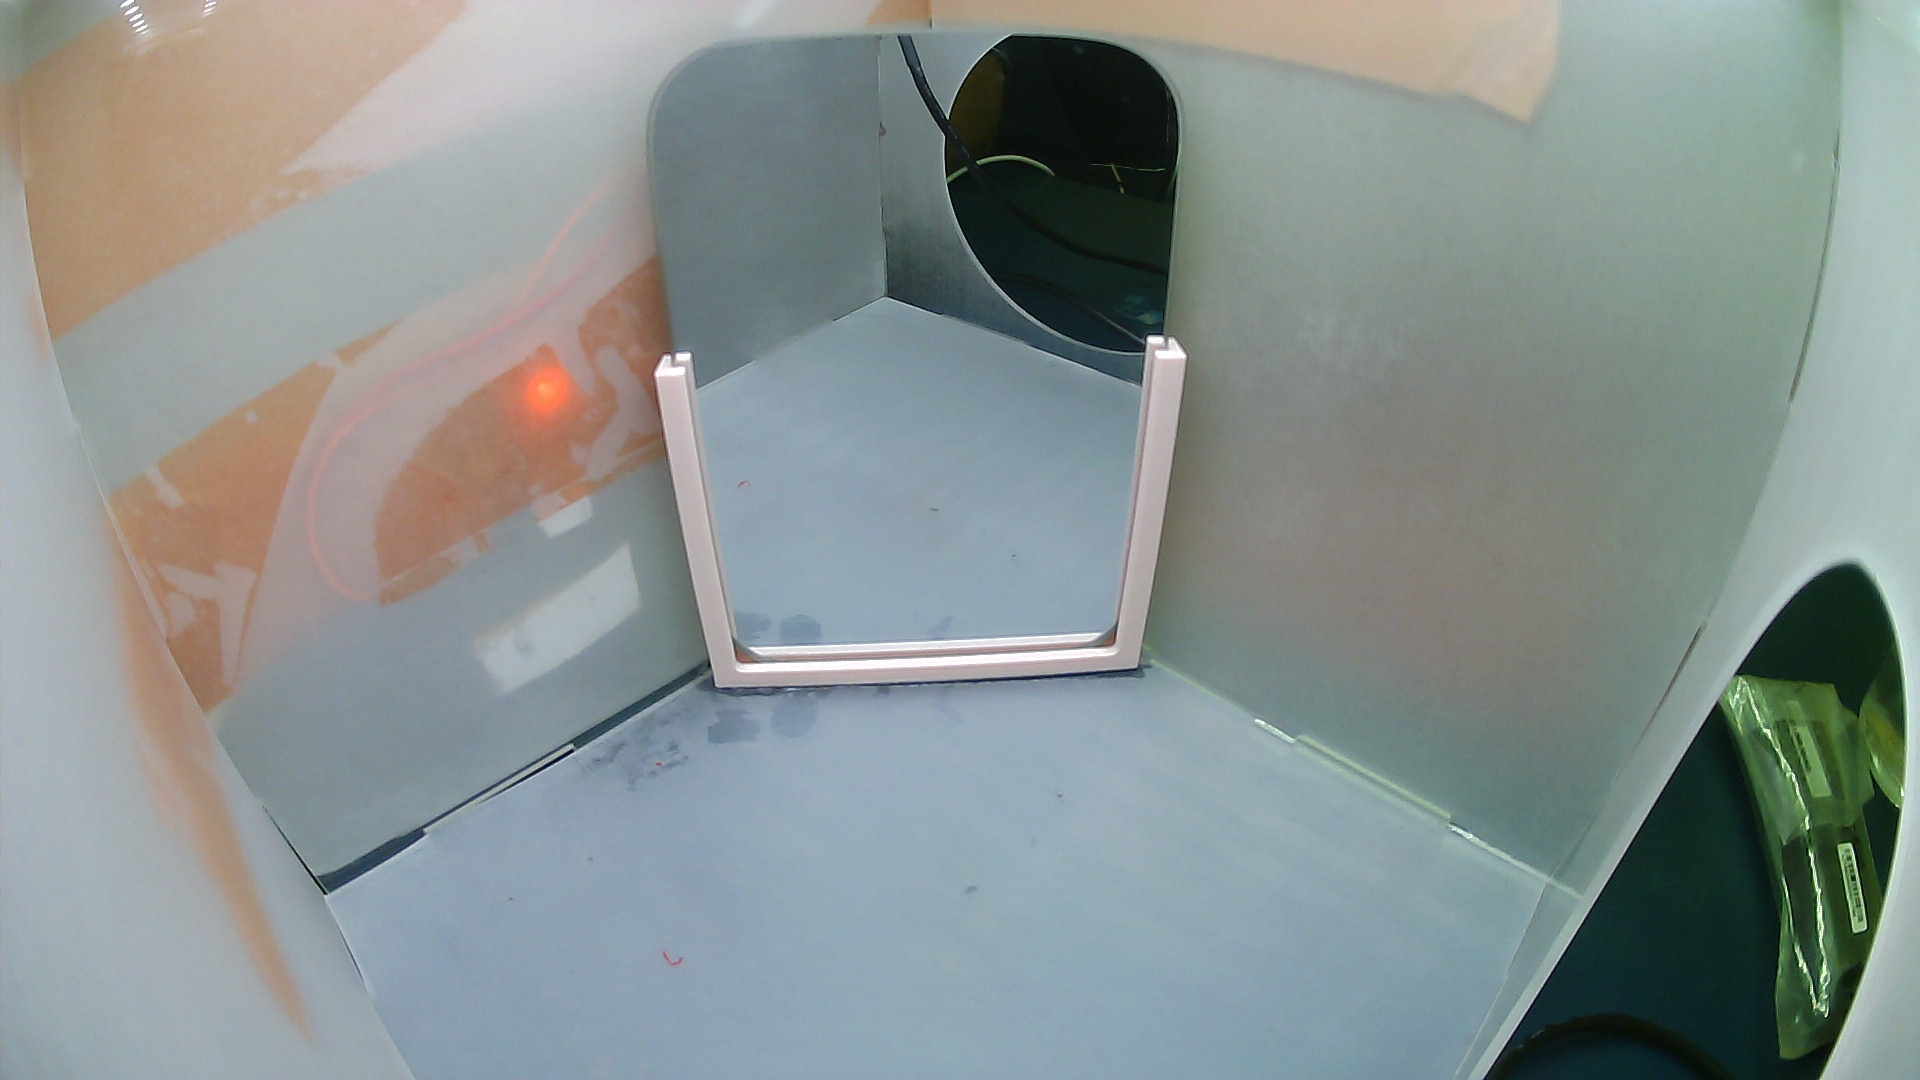
\includegraphics[width=0.6\linewidth]{images/chamber_lighting.jpg}
    \caption{Empty chamber under the fixed white lighting preset.}
    \label{fig:chamber-lighting}
\end{figure}

\chapter{Model Fine-Tuning}

This chapter describes the training and evaluation of the final three-class tomato detection model (unripe, ripe, and overripe) using the chamber dataset described in Chapter~4.

\section{Train/Validation Split by Tomato}

An important methodological correction was made when preparing the final training and validation datasets. In an initial split, individual \emph{frames} were randomly assigned to either the training or validation set. This meant that different rotational views of the same physical tomato could appear in both sets. Since the six views of a tomato share similar visual characteristics, the model could perform well on the validation set simply because it had already encountered the same tomato during training, albeit from a different angle. This would inflate the validation metrics without providing a reliable measure of generalization to previously unseen tomatoes.

To avoid this, the dataset was split at the level of individual tomatoes rather than frames. All six views of a given tomato were assigned entirely to either the training set or the validation set, ensuring that no physical tomato appeared in both.

\begin{table}[H]
    \centering
    \begin{tabular}{|l|c|c|c|}
        \hline
        \textbf{Class} & \textbf{Tomatoes (Train / Val)} & \textbf{Train Frames} & \textbf{Val Frames} \\
        \hline
        Unripe & 6 / 1 & 36 & 6 \\
        Ripe & 9 / 2 & 54 & 12 \\
        Overripe & 7 / 1 & 42 & 6 \\
        \hline
    \end{tabular}
    \caption{Final training and validation split at the tomato level.}
    \label{tab:final-dataset-split}
\end{table}

\section{Training Configuration}

A YOLO11n model, initialized from COCO-pretrained weights, was fine-tuned on the prepared chamber dataset using an input resolution of $640 \times 640$ for 80 epochs. This approach was adopted in place of continuing from the MTP-1 model, since the earlier model had been trained on the mismatched, black-background dataset discussed in Chapter~3.

\begin{table}[H]
    \centering
    \begin{tabular}{|l|c|}
        \hline
        \textbf{Metric} & \textbf{Value} \\
        \hline
        Precision & 0.981 \\
        Recall & 0.986 \\
        mAP50 & 0.981 \\
        mAP50-95 & 0.944 \\
        \hline
    \end{tabular}
    \caption{Validation metrics of the final model at epoch 80.}
    \label{tab:final-model-metrics}
\end{table}

The normalized confusion matrix in Figure~\ref{fig:normalized-confusion-matrix} provides a class-wise view of the model's predictions on the held-out validation set.

\begin{figure}[H]
    \centering
    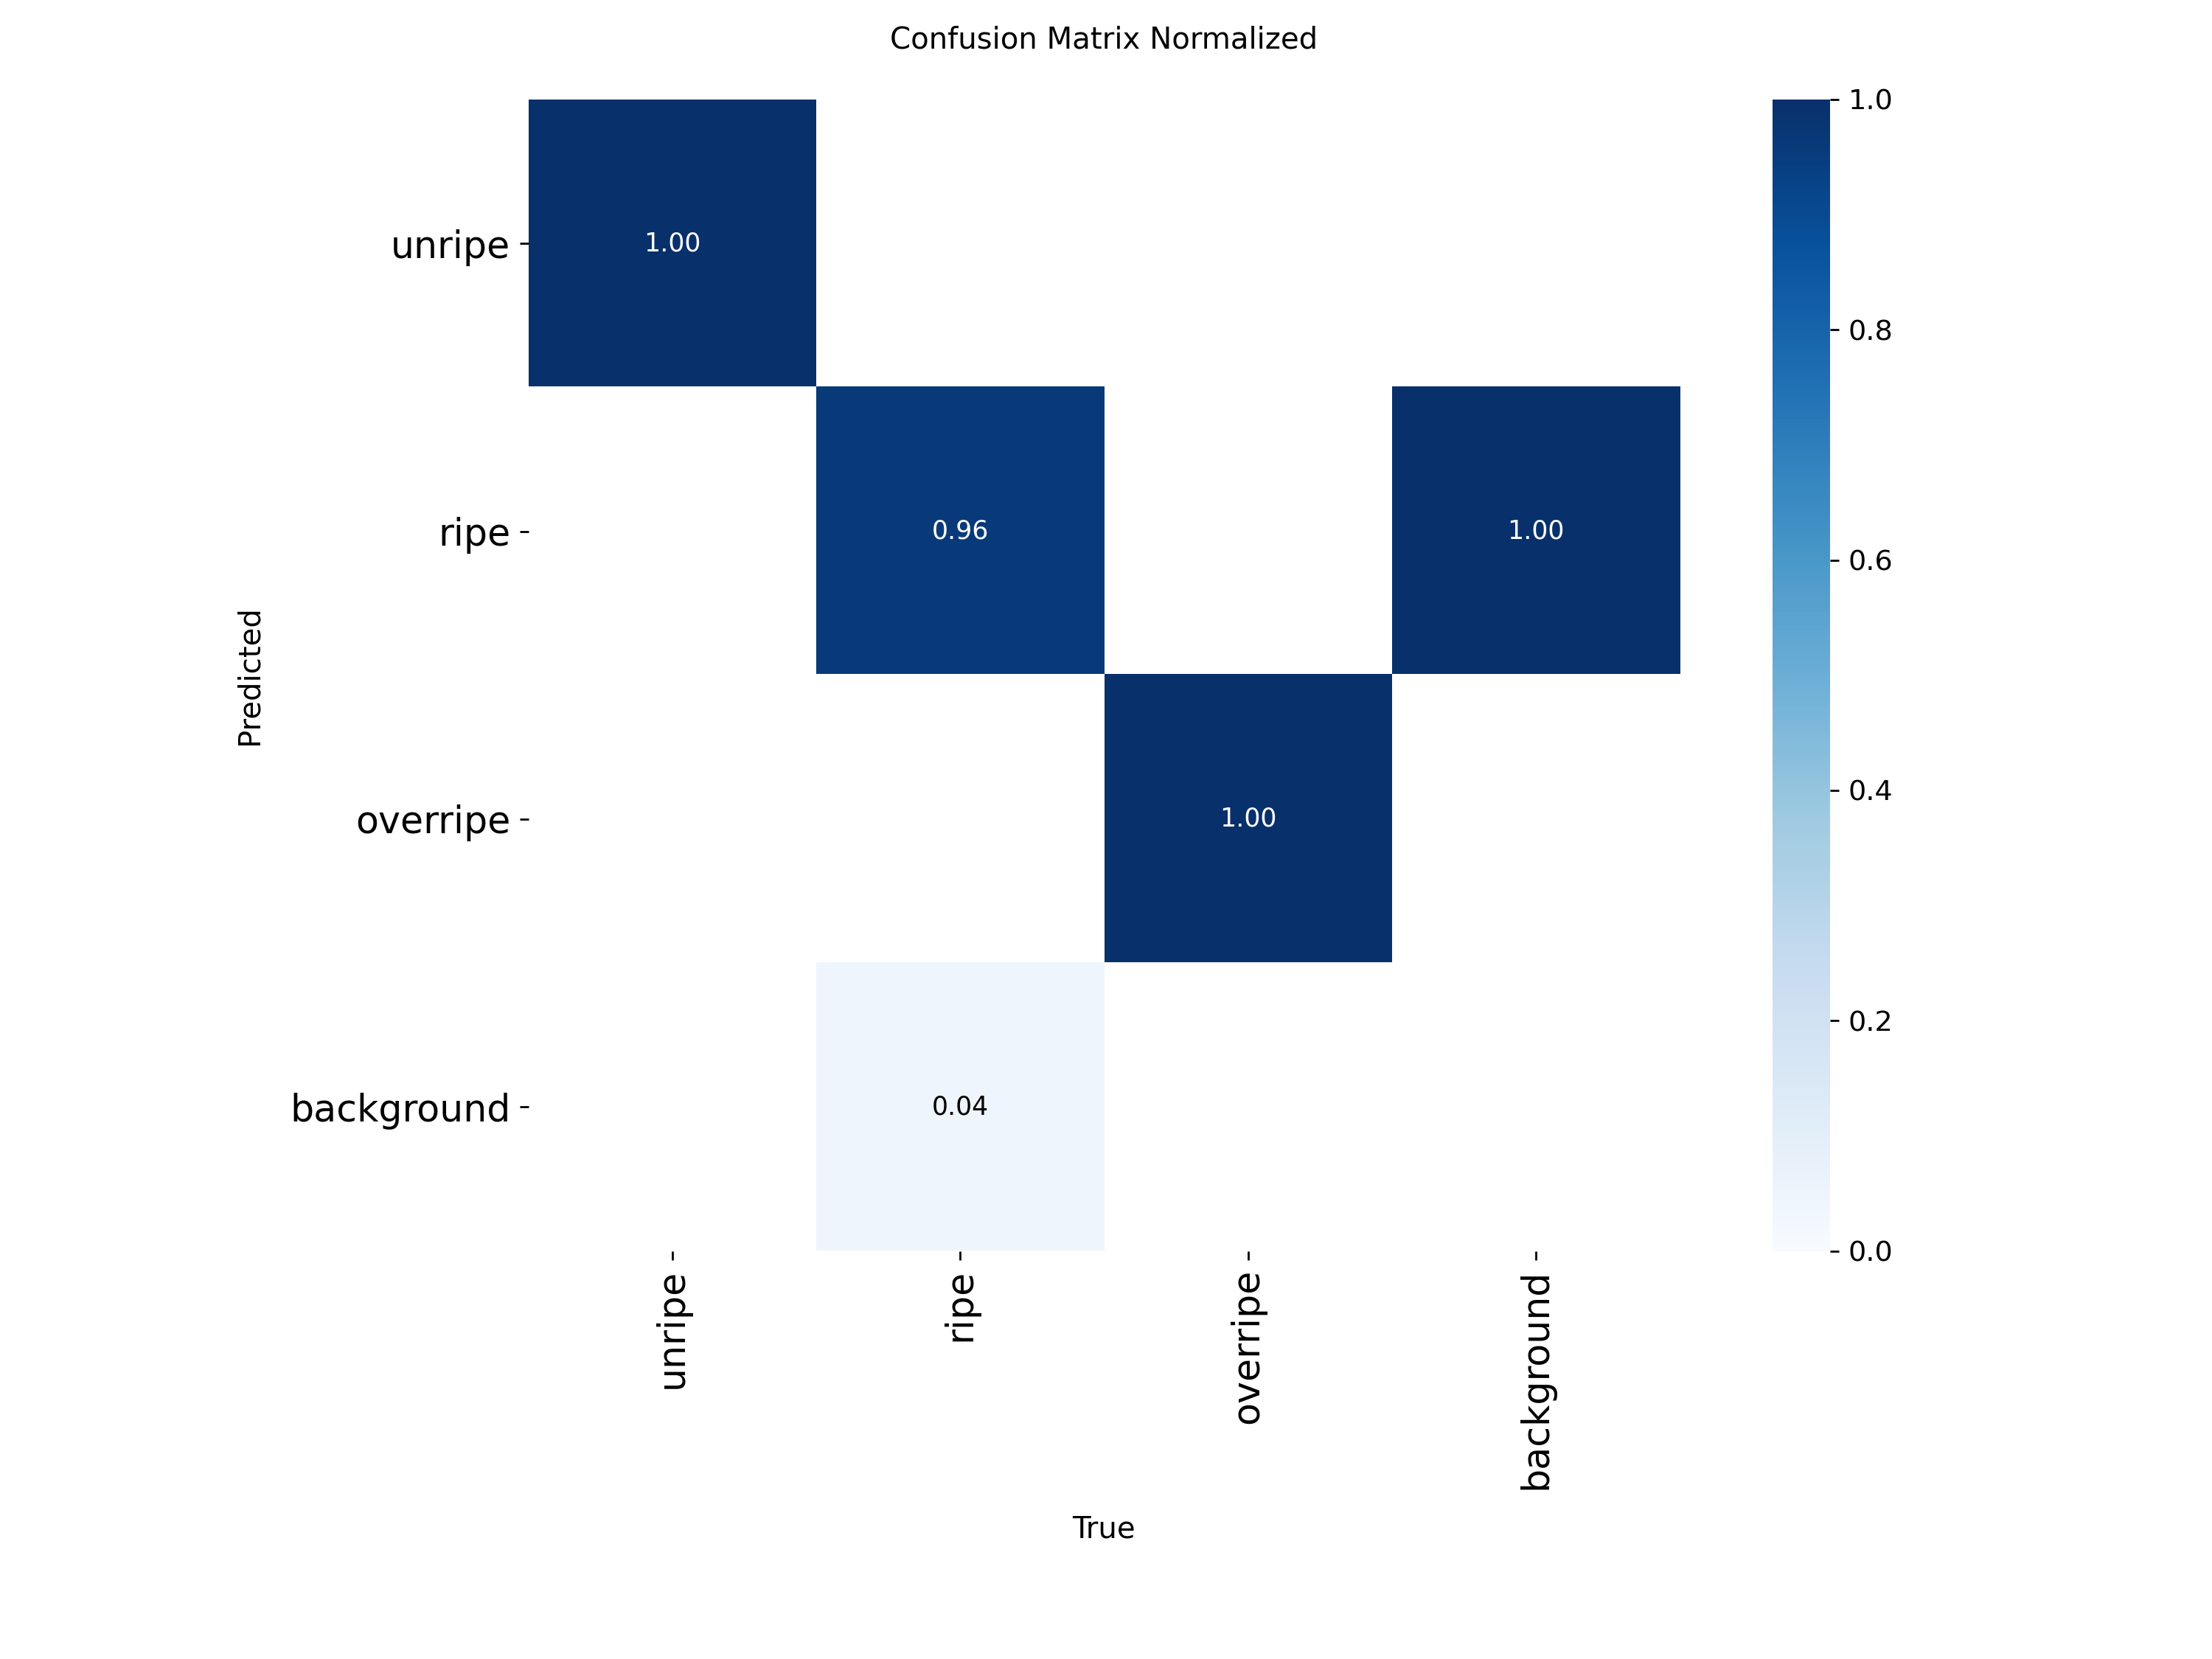
\includegraphics[width=0.75\linewidth]{images/confusion_matrix_normalized.png}
    \caption{Normalized confusion matrix on the same-session held-out validation set.}
    \label{fig:normalized-confusion-matrix}
\end{figure}

The confusion matrix shows a strongly diagonal pattern, with the unripe and overripe classes almost perfectly separated from one another and from the ripe class. The small amount of off-diagonal mass is concentrated on the ripe class, consistent with the fragile ripe/overripe boundary discussed in Chapter~3, and with a small fraction of ripe instances not receiving a confident detection at all -- consistent with the precision and recall values reported in Table~\ref{tab:final-model-metrics} above. The training and validation loss and metric curves underlying this result are shown in Figure~\ref{fig:training-curves} on the following page.

\begin{figure}[H]
    \centering
    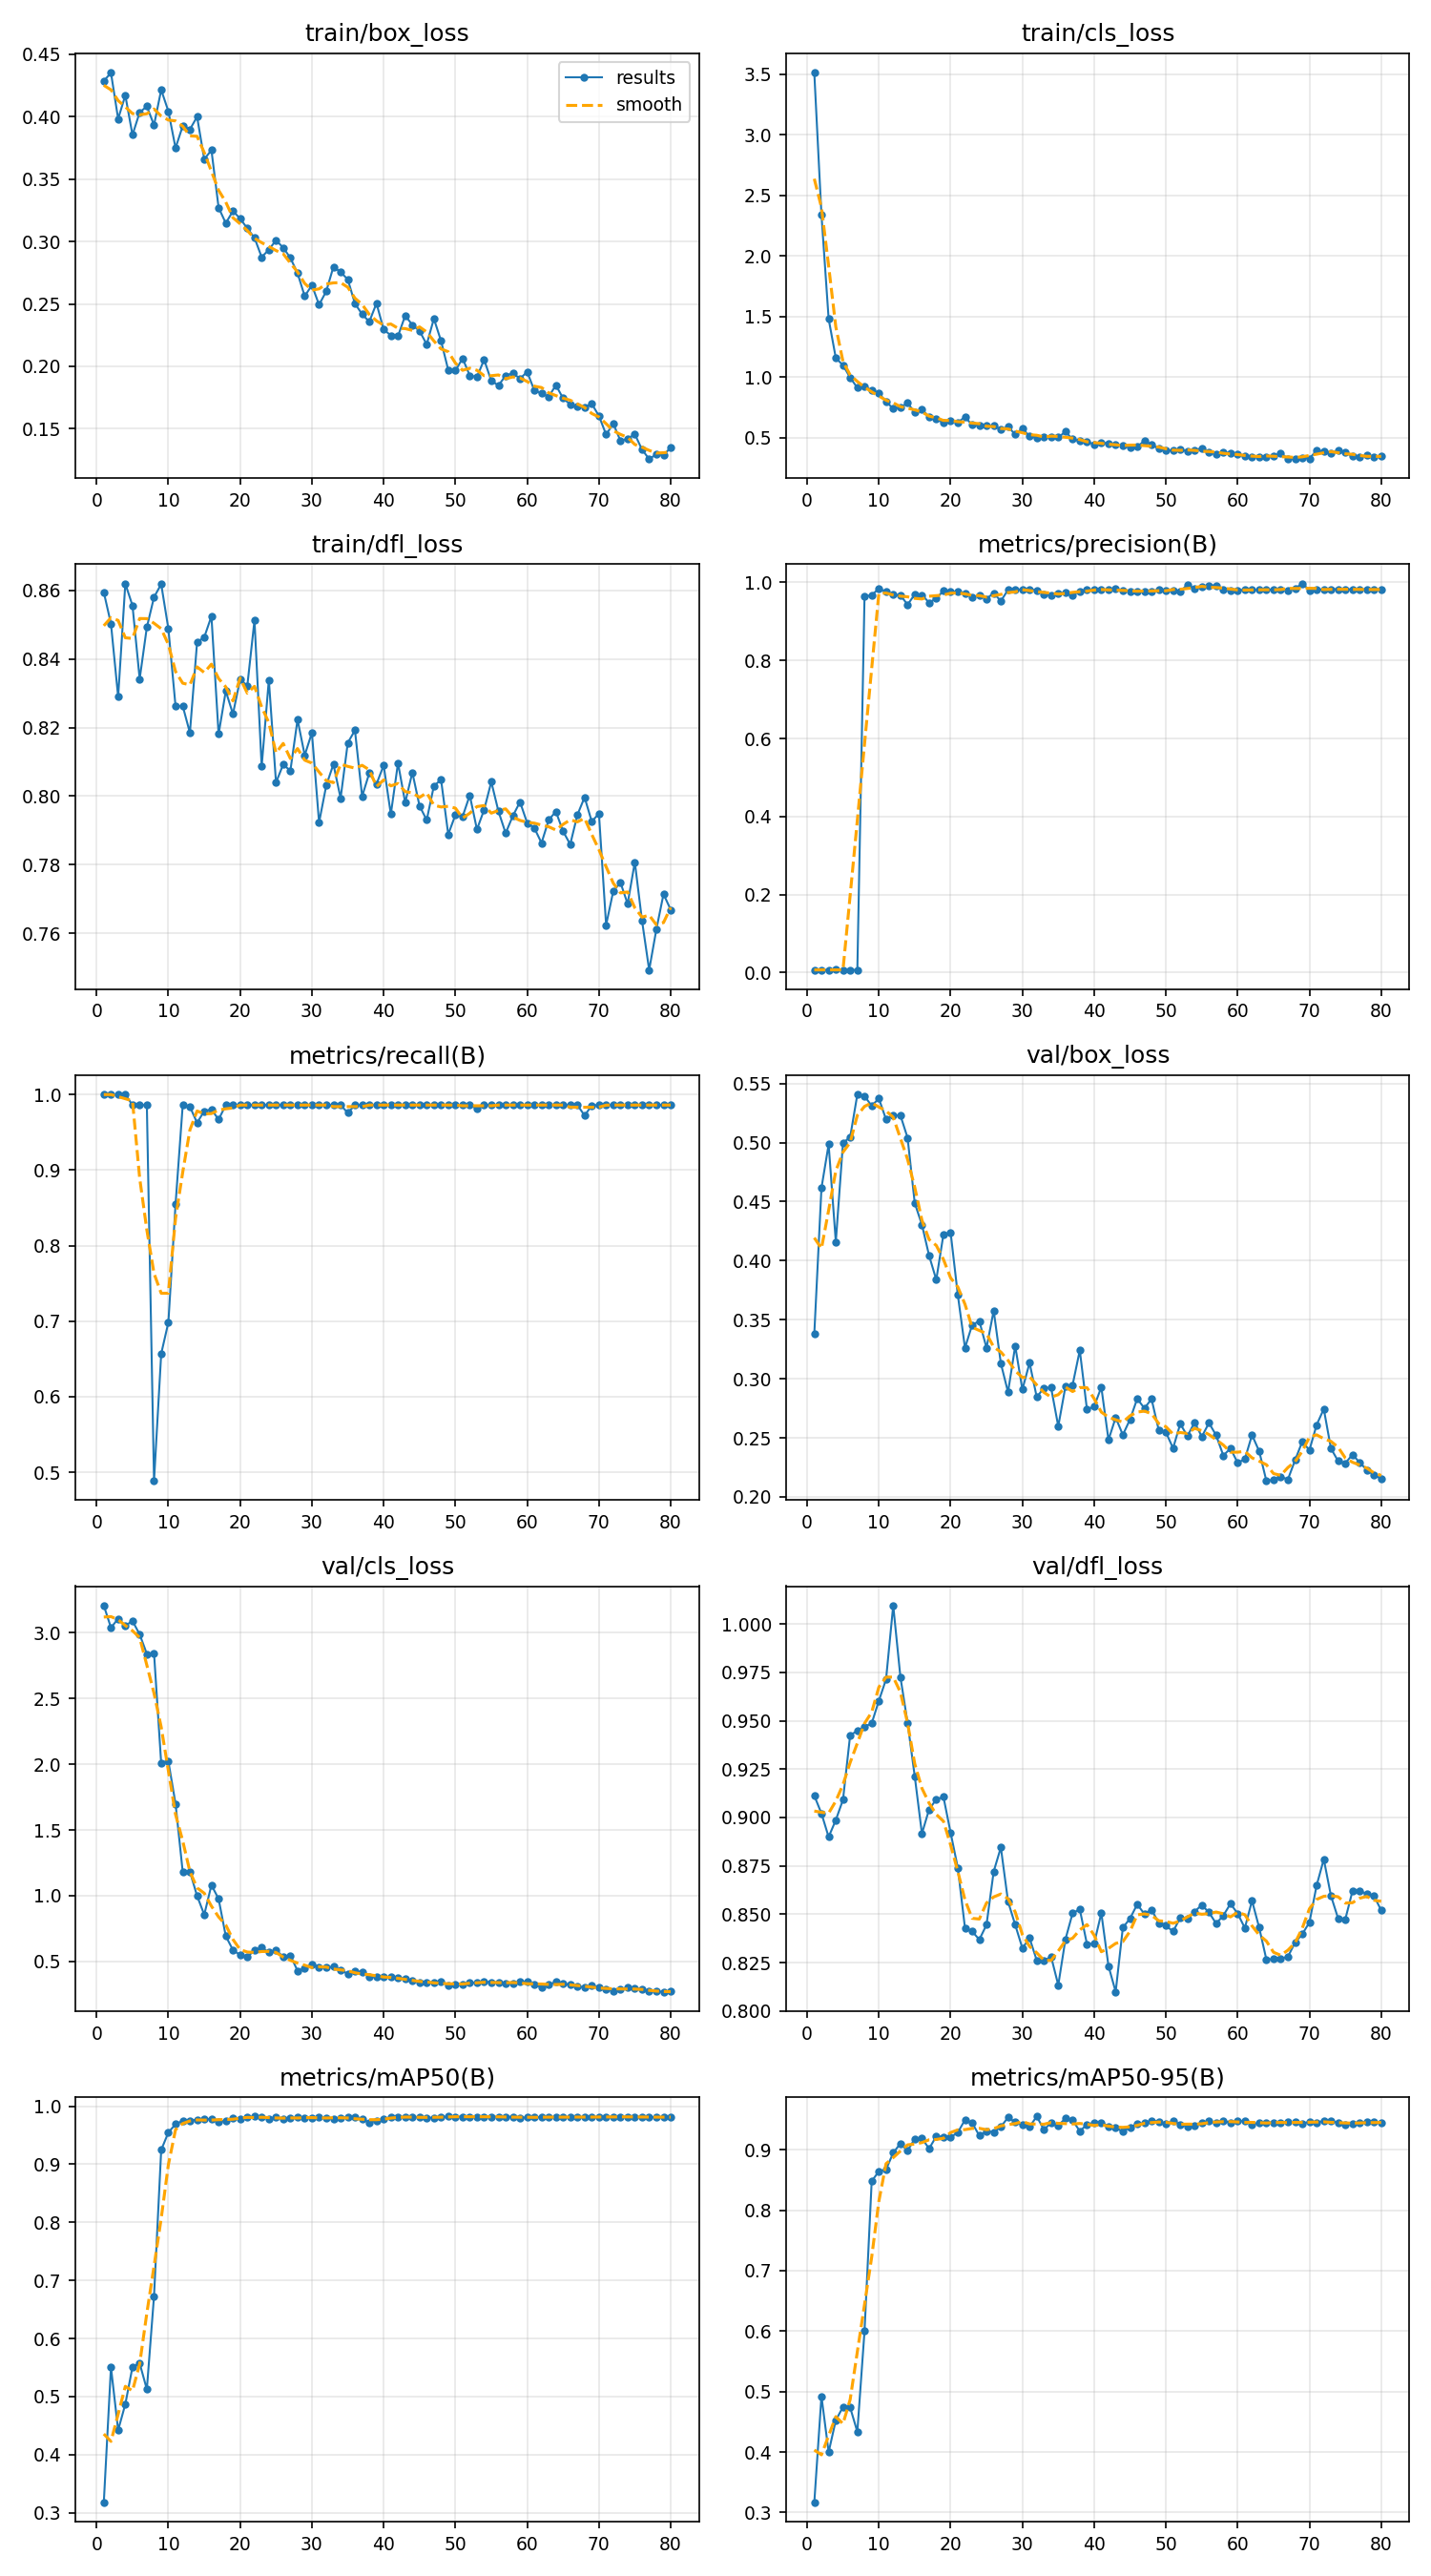
\includegraphics[width=0.85\linewidth]{images/training_curves.png}
    \caption{Training and validation loss and metric curves for the final three-class model.}
    \label{fig:training-curves}
\end{figure}

\chapter{Evaluation and Generalization Testing}

This chapter examines whether the fine-tuned model generalizes to tomatoes captured in independent data collection sessions. While the tomato-level split described in Chapter~5 prevents the same physical tomato from appearing in both the training and validation sets, both sets were captured under the same session conditions. Consequently, the validation results alone do not establish how well the model performs on previously unseen tomatoes captured during different sessions. To investigate this, the final model was evaluated on independently collected chamber images.

\section{Cross-Session Test Results}

To evaluate generalization across all three ripeness classes, an independent test set was prepared using a completely new batch of tomatoes, distinct from those used during training. The batch consisted of 10 ripe, 10 unripe, and 8 overripe tomatoes, resulting in 168 frames in total. These images were captured on a separate day under the same chamber lighting protocol. The tomatoes were visually verified to be physically distinct from those used in training, based on differences in skin texture and blemish patterns.

Each frame in this test was evaluated independently, without aggregating confidence scores across the six views of a tomato. This provides a measure of single-frame classification performance rather than a fused per-tomato decision.

\begin{table}[H]
    \centering
    \begin{tabular}{|l|c|c|}
        \hline
        \textbf{Class} & \textbf{Frames} & \textbf{Accuracy} \\
        \hline
        Unripe & 60 & 58/60 (96.7\%) \\
        Ripe & 60 & 57/60 (95.0\%) \\
        Overripe & 48 & 46/48 (95.8\%) \\
        \hline
        \textbf{Overall} & \textbf{168} & \textbf{161/168 (95.8\%)} \\
        \hline
    \end{tabular}
    \caption{Per-frame classification accuracy on the final independent cross-session test set.}
    \label{tab:cross-session-accuracy}
\end{table}

The corresponding confusion matrix is presented in Figure~\ref{tab:cross-session-confusion}. Rows represent the ground-truth classes, while columns represent the model's predicted classes.

\begin{figure}[H]
    \centering
    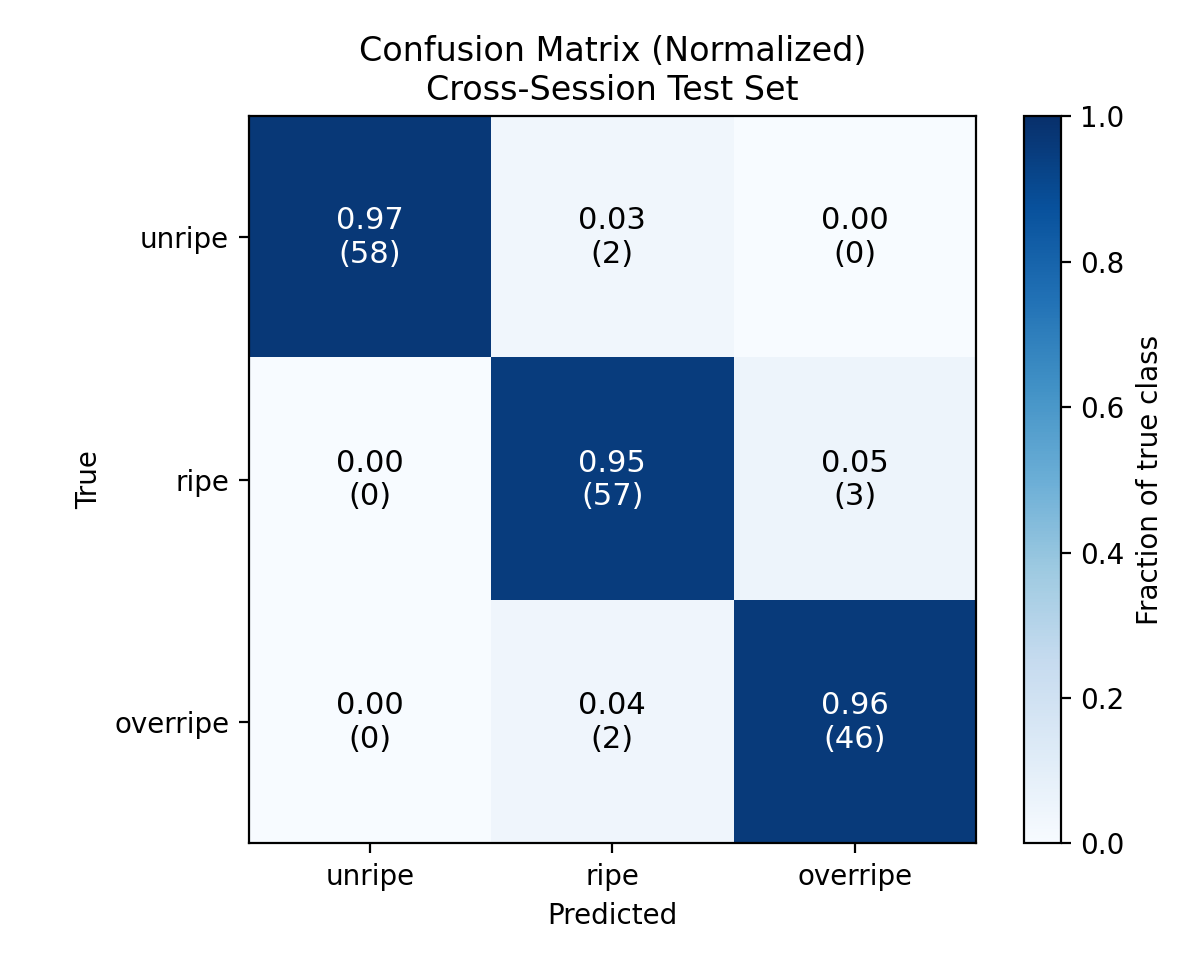
\includegraphics[width=0.65\linewidth]{images/cross_session_confusion_matrix.png}
    \caption{Confusion matrix for the final cross-session test set.}
    \label{tab:cross-session-confusion}
\end{figure}

Table~\ref{tab:cross-session-class-metrics} presents the corresponding precision, recall, and F1-score for each class.

\begin{table}[H]
    \centering
    \begin{tabular}{|l|c|c|c|c|}
        \hline
        \textbf{Class} & \textbf{Precision} & \textbf{Recall} & \textbf{F1-score} & \textbf{Support} \\
        \hline
        Unripe & 1.000 & 0.967 & 0.983 & 60 \\
        Ripe & 0.934 & 0.950 & 0.942 & 60 \\
        Overripe & 0.939 & 0.958 & 0.949 & 48 \\
        \hline
    \end{tabular}
    \caption{Per-class precision, recall, and F1-score on the final cross-session test set.}
    \label{tab:cross-session-class-metrics}
\end{table}

Of the seven misclassified frames, five involved confusion between the ripe and overripe classes: three ripe frames were predicted as overripe, while two overripe frames were predicted as ripe. This is consistent with the difficulty in distinguishing these two classes identified during the earlier diagnostic experiments in Chapter~3. The remaining two errors came from a single unripe tomato, for which two frames were predicted as ripe.

\section{Interpreting These Results}

The same-session validation mAP50-95 of 0.944 reported in Chapter~5 reflects performance on tomatoes from the same data collection session as training. Evaluating on an independent, cross-session batch provides a stronger test of generalization, since tomatoes from the same session can share incidental visual similarities that a model could exploit without genuinely learning the underlying ripeness distinction. The final independent test achieved 95.8\% accuracy across 168 images, with errors concentrated on the ripe/overripe boundary, supporting cross-session generalization.

\chapter{Edge Deployment on Raspberry Pi}

This chapter describes the deployment of the final fine-tuned model on a Raspberry Pi 4. It covers the hardware selection, model export and prediction parity verification, inference performance benchmarking, evaluation of INT8 quantization, and implementation of an event-triggered inference approach.

\section{Hardware Selection}

Two single-board computers were considered for deployment. The Raspberry Pi Zero W, which was initially available, was assessed based on its specifications: a single-core 1 GHz ARMv6 processor and 512 MB of RAM. Its processor architecture is not supported by current PyTorch builds, making it unsuitable for the intended inference setup. This was not verified through an actual inference experiment, as the only available SD card for this board failed during setup.

A Raspberry Pi 4 Model B with 8 GB of RAM and a quad-core 64-bit ARM Cortex-A72 processor was therefore used for deployment. All hardware performance measurements and deployment results presented in this chapter are based on this board.

\section{Model Export and Parity Verification}

The final PyTorch model was exported to NCNN format at full 32-bit floating-point (FP32) precision. NCNN is a lightweight inference framework designed to support efficient neural network execution on CPU-based devices, including ARM platforms.

Before evaluating inference performance on the Raspberry Pi, the exported model was compared against the original PyTorch model using seven held-out test frames. This was done to verify that the export process had preserved the model's predictions. Both implementations correctly classified all seven frames and produced identical top-ranked classes. The confidence scores also showed close agreement, differing by no more than 0.01 on six of the seven frames.

In terms of inference speed, the PyTorch model on the PC achieved a mean latency of 16 ms, while the NCNN model on the Raspberry Pi 4 took 389 ms per frame. These results indicate that the export process preserved the model's prediction behaviour on the tested samples, with the main difference being inference latency, driven by the Raspberry Pi's more limited computational resources and the absence of GPU acceleration.

\section{Thread-Count Tuning}

NCNN supports multi-threaded inference, allowing it to utilize multiple CPU cores on the Raspberry Pi. Since the number of threads can affect inference latency, experiments were conducted with different thread counts. These measurements were obtained by calling the NCNN library directly, bypassing the higher-level Python wrapper, which did not reliably expose the thread-count setting.

\begin{table}[H]
    \centering
    \begin{tabular}{|c|c|c|}
        \hline
        \textbf{Threads} & \textbf{Mean Latency} & \textbf{FPS} \\
        \hline
        1 & 680 ms & 1.47 \\
        2 & 440 ms & 2.27 \\
        3 & 405 ms & 2.47 \\
        4 & 362 ms & 2.76 \\
        \hline
    \end{tabular}
    \caption{NCNN inference latency for different CPU thread counts on the Raspberry Pi 4.}
    \label{tab:ncnn-threads}
\end{table}

Increasing the number of threads improved inference speed, with the largest improvement observed when moving from one to two threads. Using all four CPU cores reduced the mean latency from 680 ms to 362 ms, nearly doubling the inference throughput compared with single-threaded execution. However, the improvements became smaller beyond two threads. The four-thread configuration, which achieved a mean latency of 362 ms per inference, was selected for subsequent deployment experiments.

\section{INT8 Quantization: Evaluated and Rejected}

As a further optimization, the model was also exported to TensorFlow Lite (TFLite) using full INT8 quantization. This represents model weights and activations using 8-bit integers instead of 32-bit floating-point values, potentially reducing memory requirements and computational cost.

The quantized model was benchmarked on the Raspberry Pi using the same seven held-out frames used for the earlier parity evaluation, and its performance was compared with the thread-tuned NCNN FP32 model. The NCNN FP32 model achieved a mean latency of 362 ms and classified all held-out frames correctly, including the ripe class. The TFLite INT8 model, by contrast, was slower, with a mean latency of 484 ms, and it also ranked ``overripe'' above ``ripe'' on one held-out ripe frame, a misclassification the FP32 model did not make. The TFLite INT8 model was therefore slower than the NCNN FP32 model on the Raspberry Pi, despite the theoretical computational advantages of integer arithmetic -- likely due to differences in how the two inference frameworks are optimized for this hardware.

The quantization process used a calibration set of 24 images, which may have been insufficient to represent the variation in the dataset accurately. Given the slower observed inference time and the prediction difference near the already-sensitive ripe/overripe boundary, INT8 quantization was not adopted. The NCNN FP32 model was retained for deployment.

\section{Event-Triggered Inference}

An important design requirement was to avoid running the detection model continuously. Instead, inference should be initiated only when a tomato is ready to be classified, with successive classification events separated in time. Two complementary triggering modes were implemented to support this requirement.

\textbf{Manual-trigger mode} performs no camera polling or model inference while the system is idle. A classification sequence begins only after an explicit user input. Once triggered, the system captures six views at one-second intervals, allowing the tomato to be rotated between successive captures. The confidence scores for each class are accumulated across all six views, and the class with the highest cumulative score is selected as the final prediction. This follows the multi-view fusion principle used in the Stage-1 mobile application described in Chapter~2, adapted to the detection model's confidence outputs.

\textbf{Automatic-trigger mode} uses a lightweight presence-detection mechanism to identify when a tomato has been placed inside the chamber. It compares the saturation and frame-to-frame motion of downsampled camera frames against a calibrated empty-chamber baseline. These checks run several times per second without invoking the detection model. Model inference is triggered only when a tomato is detected as present and remains stationary for a sustained period, thereby filtering out transient motion caused by a hand placing the tomato. After a classification event, the system does not trigger again until the chamber is detected as empty.

During testing, the automatic-trigger mechanism initiated a single classification event for each tomato placed in the chamber and ignored the motion associated with placing or removing a tomato. The detection model was active for only a small fraction of the total runtime, demonstrating that the event-triggered approach avoids unnecessary continuous inference.

\chapter{Results}

This chapter consolidates the key findings from the development and evaluation of the automated tomato sorting system. It brings together the results of the Stage-1 model diagnosis, training and evaluation of the final three-class detection model, and its deployment on the Raspberry Pi 4.
\section{Diagnosis of the Stage-1 Model}

The diagnostic experiments revealed significant limitations in the Stage-1 model's performance on actual chamber images. During the live empty-chamber test, the model produced a false-positive detection, classifying the empty chamber as ``unripe'' with a confidence of 0.97. To investigate the poor performance on ripe tomatoes, YOLO11n and YOLO11s were evaluated on the same chamber images. Both performed similarly, achieving accuracies of 20.8\% and 18.8\%, respectively, suggesting that increasing model size alone would not resolve the problem.

A further experiment examined whether background mismatch was the primary cause. Chamber images were reprocessed by segmenting the tomatoes and replacing their backgrounds with black, following the Stage-1 preprocessing approach. However, ripe-class accuracy dropped to 0\%, indicating that background mismatch alone was insufficient to explain the failure.

Visual comparison revealed that Stage-1 images labelled as ``ripe'' predominantly contained dull orange or amber tomatoes, whereas chamber-captured ripe tomatoes had a more vivid red appearance, closer to the Stage-1 ``overripe'' examples. Along with differences in tomato scale and framing, this highlighted a mismatch between the original training data and the actual chamber environment, motivating the collection of a new chamber-specific dataset.
\section{Final Model Performance}

The final three-class YOLO11n model was trained using the chamber dataset, with separate training and validation sets at the tomato level to prevent different views of the same physical tomato from appearing in both sets and achieved a validation mAP50-95 of 0.944. However, an initial independent evaluation revealed that none of the six held-out ripe tomatoes were classified correctly. Following the addition of three new ripe tomatoes to the training dataset, the model was evaluated on the remaining held-out samples, showing an improvement in ripe-class predictions.

The final model was subsequently evaluated on a separate cross-session test set containing 168 frames from 28 previously unseen tomatoes. It correctly classified 58 out of 60 unripe frames (96.7\%), 57 out of 60 ripe frames (95.0\%), and 46 out of 48 overripe frames (95.8\%). Overall, the model correctly classified 161 out of 168 frames, achieving an accuracy of 95.8\%.

Most errors occurred between the ripe and overripe classes, while the unripe class was distinguished more consistently. All three classes achieved F1-scores above 0.94. These results demonstrate improved performance across independently captured sessions under the same chamber setup and lighting protocol, although distinguishing visually similar ripeness stages remains challenging.

\section{Edge Deployment Performance}

The final model was deployed on the Raspberry Pi 4 using the NCNN inference framework at full FP32 precision. The original PyTorch model occupied approximately 5.2 MB, while the exported NCNN model occupied approximately 10 MB. Prediction parity was verified using seven held-out frames, with both implementations producing identical top-ranked classifications on all seven frames. Their confidence scores also remained close, differing by no more than 0.01 on six of the seven frames.

Inference benchmarking showed that using four CPU threads achieved the best measured latency of 362 ms per frame, corresponding to approximately 2.76 FPS. An alternative deployment using TFLite INT8 quantization was also evaluated but recorded a higher latency of 484 ms and produced an incorrect class ranking on one held-out ripe frame. Consequently, the NCNN FP32 implementation was retained.

An event-triggered inference mechanism was also implemented to avoid unnecessary continuous execution of the detection model. The manual mode initiates classification only after explicit user input, while the automatic mode uses lightweight presence and motion checks to identify when a tomato has been placed and has become stationary. During testing, the automatic mode successfully initiated a single classification event per tomato placement while ignoring transient hand movements.

Overall, the deployment experiments demonstrated that the final model could run on the Raspberry Pi 4 while maintaining consistency with the original implementation on the tested samples. The combination of multiview inference and event-triggered execution established a practical approach for running the model on the embedded hardware.

\chapter{Conclusion and Future Work}

Stage-2 began by establishing that the near-perfect validation performance of the Stage-1 YOLO model did not translate to actual deployment performance. The experiments identified differences in tomato appearance between the training dataset and real chamber footage, along with a mismatch in object scale and framing. These findings shaped the subsequent work: an automated annotation pipeline using SAM2 was developed to label full chamber images, a three-class dataset was collected, and the data was split at the tomato level to prevent validation leakage. The resulting model was evaluated on both same-session and independent cross-session data, with the latter exposing an additional generalization gap in the ripe class that was addressed by expanding the training dataset.

The final model was deployed on a Raspberry Pi 4 using NCNN. Its predictions were verified against the original PyTorch implementation, inference performance was benchmarked and optimized through thread-count tuning, and an INT8 quantization alternative was evaluated but not adopted due to its higher latency and prediction differences. Additionally, manual and automatic event-triggered inference mechanisms were implemented to ensure that classification is performed only when required, rather than continuously.

Several aspects of the system remain open for further development. The cross-session test set can be expanded through additional capture sessions and tomato batches to establish greater confidence in the reported generalization results. This is particularly important for the overripe class, as sourcing genuinely overripe tomatoes remains logistically challenging. Further testing under sustained workloads is also required to evaluate whether inference latency remains stable during extended operation and to assess the thermal behaviour of the Raspberry Pi.

Another area for exploration is the use of a dedicated AI-accelerator camera module, such as reCamera, as a higher-performance alternative to the Raspberry Pi. A decision on this would depend on establishing the required processing throughput in terms of tomatoes classified per minute.

Finally, integration with the physical sorting mechanism remains an important step towards completing the automated system. This would enable the system to perform the complete process, from image capture and ripeness classification to the physical sorting of tomatoes.
\end{document}
